\documentclass[xcolor=table,aspectratio=169]{beamer}

% General settings
\usetheme{Madrid}
\usepackage[T1]{fontenc}
\usepackage{graphicx}

\usepackage{xskak,chessboard}

% Remove navigation symbols
\beamertemplatenavigationsymbolsempty

% Fonts
\usepackage{helvet}
\setbeamerfont{normal text}{family=helvet}
\setbeamerfont{local structure}{family=helvet}

% Colors
\definecolor{kgrey}{HTML}{2b2828}
\setbeamercolor{frametitle}{bg=kgrey,fg=white}
\setbeamercolor{block title}{bg=kgrey,fg=white}

% Lists
\setbeamertemplate{enumerate items}[default]
\setbeamertemplate{itemize items}{\normalsize $\bullet$}
\setbeamercolor{description item}{fg=kgrey}
\setbeamercolor{enumerate item}{fg=kgrey}
\setbeamercolor{itemize item}{fg=kgrey}
\setbeamercolor{itemize subitem}{fg=kgrey}
\setbeamercolor{itemize subsubitem}{fg=kgrey}

% Templates
\setbeamertemplate{blocks}[default]
\setbeamertemplate{frametitle}{}
\setbeamertemplate{footline}{}
\usepackage{tcolorbox}
\tcbuselibrary{skins,hooks}
\tcbset{colframe=structure,fonttitle=\bfseries,beamer, clip upper, boxsep=0pt, sharp corners=all, no shadow, left skip=0pt, right skip=0pt, coltext=white}
\setbeamertemplate{title page}
{
  \leavevmode%
  \vbox{%
  \vspace{-1.6ex}%
  \noindent\begin{tcolorbox}[enhanced,watermark graphics=photo.png, width=\paperwidth, height=0.575\paperwidth, watermark zoom=1.25, grow to left by=0.035\paperwidth, frame hidden]

  \vspace{7.5em}
  \begin{center} 
  \huge
  \textbf{\inserttitle}

  \end{center}
  \end{tcolorbox}

  \vspace{-2em}
  \begin{tcolorbox}[width=\paperwidth, enhanced, colback=kgrey, grow to left by=0.035\paperwidth,]
  \begin{center}
  \footnotesize \bf \insertauthor\quad | \quad \insertdate    
  \end{center}
  \end{tcolorbox}
  }
}

\title{MARVEL Pub Quiz}
\author{Edward Linscott}
\date{17 Jan 2024}
\begin{document}
\frame{\titlepage}
\begin{frame}
   The format:
   \begin{itemize}[<+(1)->]
      \item five regular rounds
      \begin{itemize}
         \item eight questions each, which we will go through together
         \item questions within each round are linked by some common thread
      \end{itemize}
      \item picture and puzzle rounds
      \begin{itemize}
         \item for you to complete in your spare time
         \item examples to follow
      \end{itemize}
   \end{itemize}

   \onslide<8->{The etiquette:}
   \begin{itemize}[<+(1)->]
      \item if you need something clarified, just ask!
      \item at the end of each round I can repeat previous questions upon request, so don't worry if you've forgotten what a previous question was
      \item the quizmaster is \emph{always} right
   \end{itemize}
\end{frame}

\begin{frame}
   Example picture

   \begin{center}
      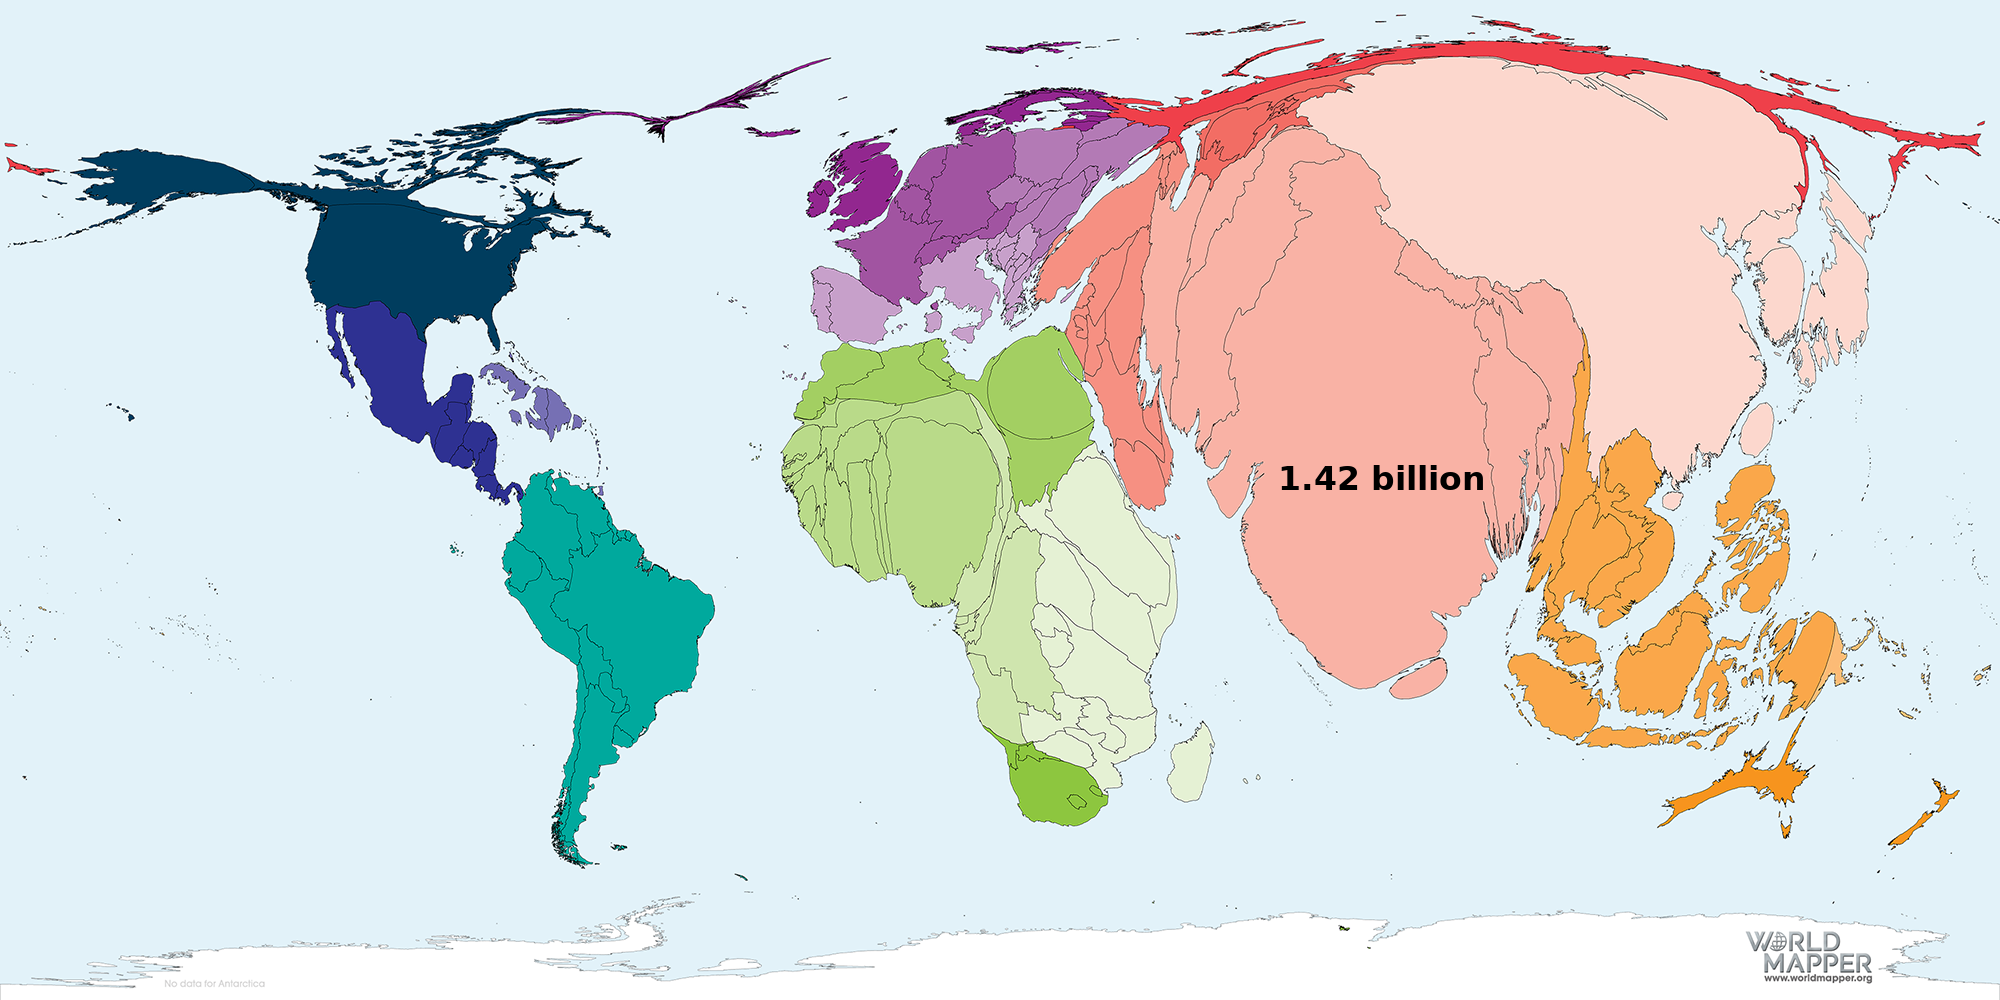
\includegraphics[width=0.6\paperwidth]{maps/population.png}

      \onslide<2->{population}
   \end{center}
\end{frame}

\begin{frame}
    \large
    Example puzzle 1. What links
          \begin{center}
                  magic, hugo, alfa, california
          \end{center}
   \onslide<2->{\textit{They all combine with a word from the NATO alphabet: Magic Mike, Victor Hugo, Alfa Romeo, and Hotel California}}
\end{frame}

\begin{frame}
   \large
   Example puzzle 2. What links
   \begin{center}
      \begin{minipage}{0.6\textwidth}
          \textit{%
              pe (skateboarding) \onslide<3->{= half-pi\textbf{pe}} \\
              thon (athletics) \onslide<4->{= half mara\textbf{thon}} \\
              son (wrestling) \onslide<5->{= half nel\textbf{son}} \\
              ley (tennis) \onslide<6->{= half-vol\textbf{ley}}}%
      \end{minipage}
   \end{center}

   \onslide<2->{Halves}%

\end{frame}

\begin{frame}
\begin{center}
\Huge
Round 1: Switzerland
\end{center}
\end{frame}
\begin{frame}
\begin{center}
\Large
1. Skiing is a very, very, old activity. The earliest evidence of skiing comes from which country?
\end{center}
\end{frame}
\begin{frame}
\begin{center}
\Large
2. In "A Big Day Out", why do Wallace and Gromit go to the moon?
\end{center}
\end{frame}
\begin{frame}
\begin{center}
\Large
3. Which 2000 romance saw Johnny Depp star as the love interest of Juliette Binoche?
\end{center}
\end{frame}
\begin{frame}
\begin{center}
\Large
4. What object has a face, a crown, and a lug?
\end{center}
\end{frame}
\begin{frame}
\begin{center}
\Large
5. Which federation was founded in 1904 by representatives from France, Belgium, Denmark, Spain, Sweden and the Netherlands?
\end{center}
\end{frame}
\begin{frame}
\begin{center}
\Large
6. This is an emblem of which organisation?
\\
\vspace{0.5em}
\includegraphics[height=0.6\paperheight]{images/red_crystal.png}
\end{center}
\end{frame}
\begin{frame}
8. Which of the following is NOT a Swiss tradition?   
\begin{itemize}
      \item cow-vs-cow fighting
      \item burning a snowman
      \item men dressing up as bushes
      \item a sport that's a cross between golf and baseball
      \item a turnip parade
      \item wrapping women in quilts
   \end{itemize}

\end{frame}
\begin{frame}
\begin{center}
\Huge
Answers
\end{center}
\end{frame}
\begin{frame}
\begin{center}
\Large
1. Skiing is a very, very, old activity. The earliest evidence of skiing comes from which country?
\\
\onslide<2->{\vspace{1em}\textit{Russia}}
\end{center}
\end{frame}
\begin{frame}
\begin{center}
\Large
2. In "A Big Day Out", why do Wallace and Gromit go to the moon?
\\
\onslide<2->{\vspace{1em}\textit{to get some cheese}}
\end{center}
\end{frame}
\begin{frame}
\begin{center}
\Large
3. Which 2000 romance saw Johnny Depp star as the love interest of Juliette Binoche?
\\
\onslide<2->{\vspace{1em}\textit{Chocolat}}
\end{center}
\end{frame}
\begin{frame}
\begin{center}
\Large
4. What object has a face, a crown, and a lug?
\\
\onslide<2->{\vspace{1em}\textit{A watch}}
\end{center}
\end{frame}
\begin{frame}
\begin{center}
\Large
5. Which federation was founded in 1904 by representatives from France, Belgium, Denmark, Spain, Sweden and the Netherlands?
\\
\onslide<2->{\vspace{1em}\textit{FIFA}}
\end{center}
\end{frame}
\begin{frame}
\begin{center}
\Large
6. This is an emblem of which organisation?
\\
\only<1>{\vspace{0.5em}
\includegraphics[height=0.6\paperheight]{images/red_crystal.png}}
\only<2>{\vspace{0.5em}
\includegraphics[height=0.3\paperheight]{images/red_cross_cresent_crystal.png}}
\\
\onslide<2->{\vspace{1em}\textit{The Red Cross}}
\end{center}
\end{frame}
\begin{frame}
\begin{columns}
\begin{column}{0.5\paperwidth}
   8. Which of the following is NOT a Swiss tradition?   
\begin{itemize}
      \item cow-vs-cow fighting
      \item burning a snowman
      \item men dressing up as bushes
      \item a sport that's a cross between golf and baseball
      \item a turnip parade
      \item wrapping women in quilts
   \end{itemize}

\end{column}
\begin{column}{0.4\paperwidth}
   \begin{overlayarea}{\columnwidth}{0.6\paperheight}
      \only<2>{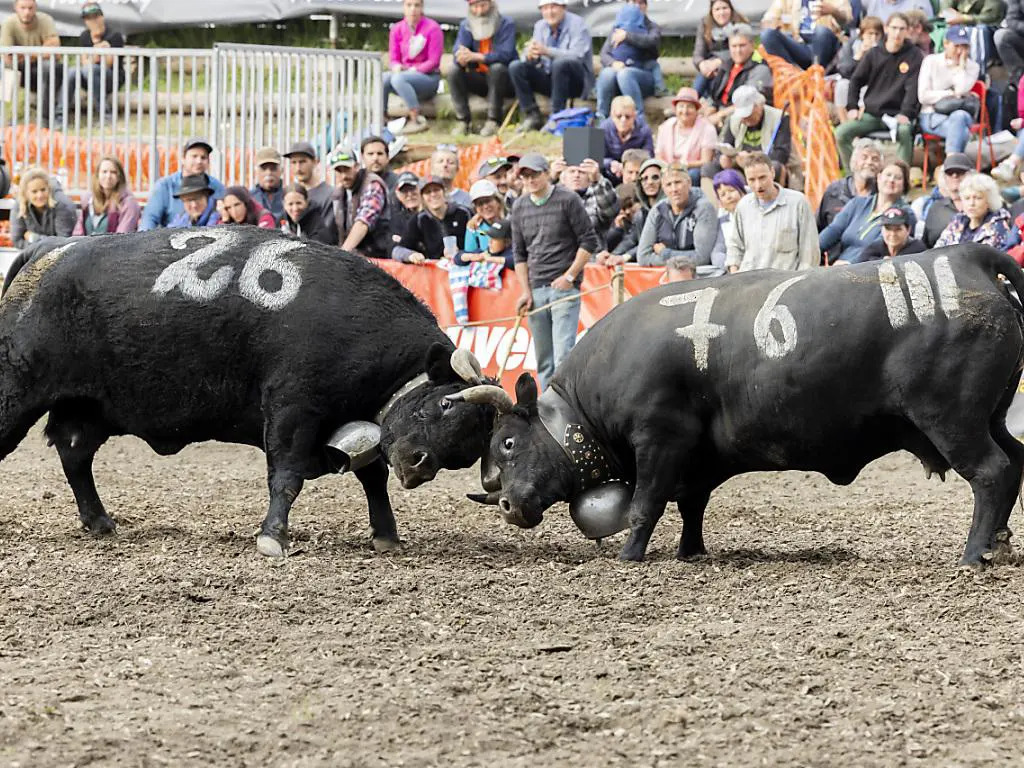
\includegraphics[width=\columnwidth]{images/cow_fighting.jpg}}
      \only<3>{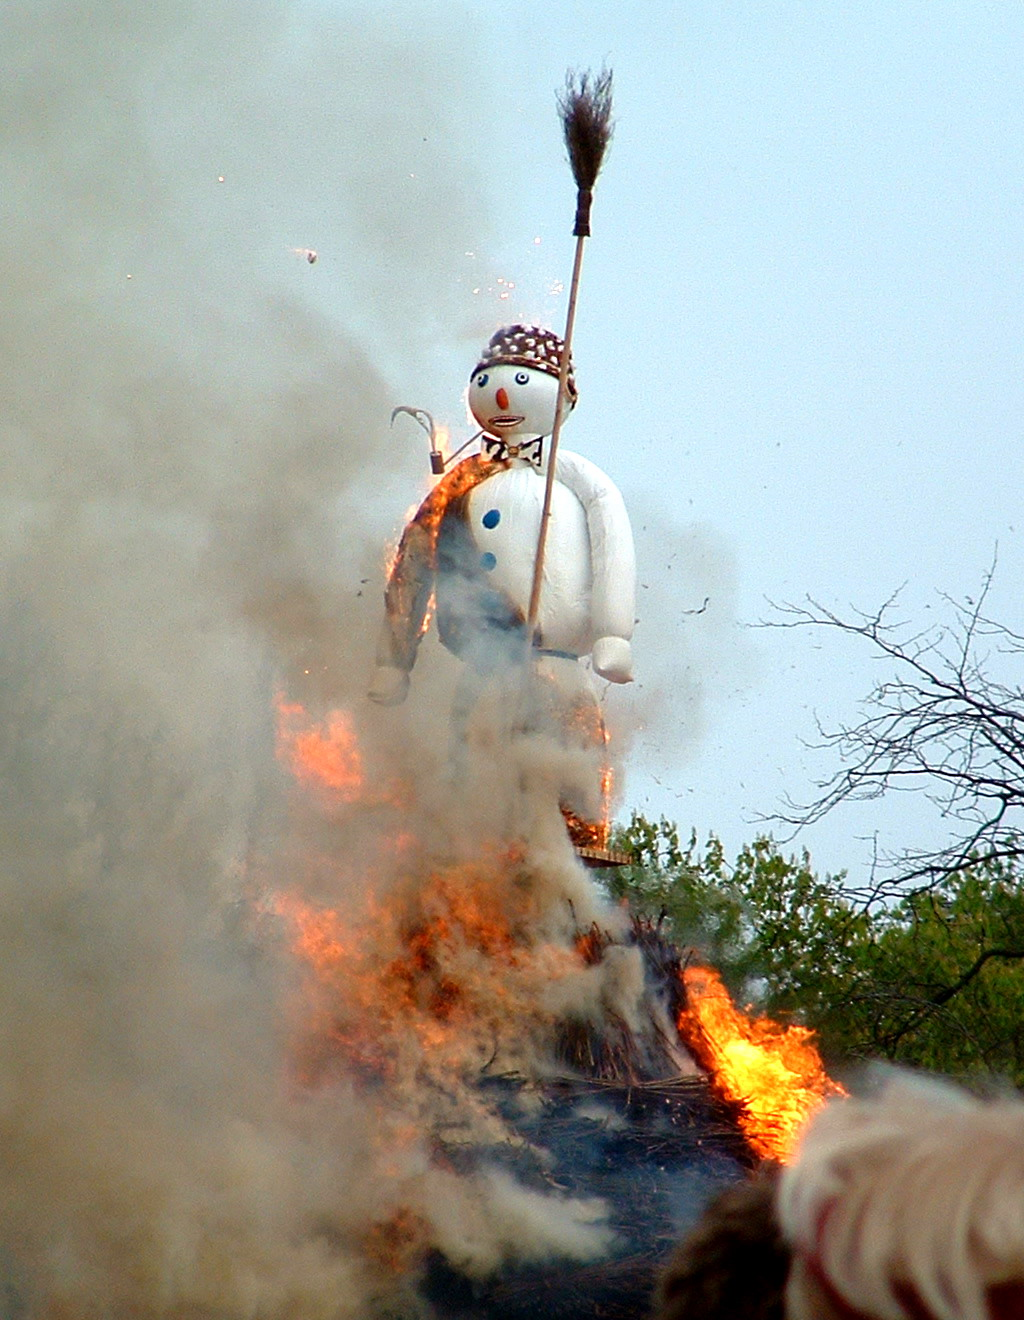
\includegraphics[height=0.6\paperheight]{images/boogg.jpg}}
      \only<4>{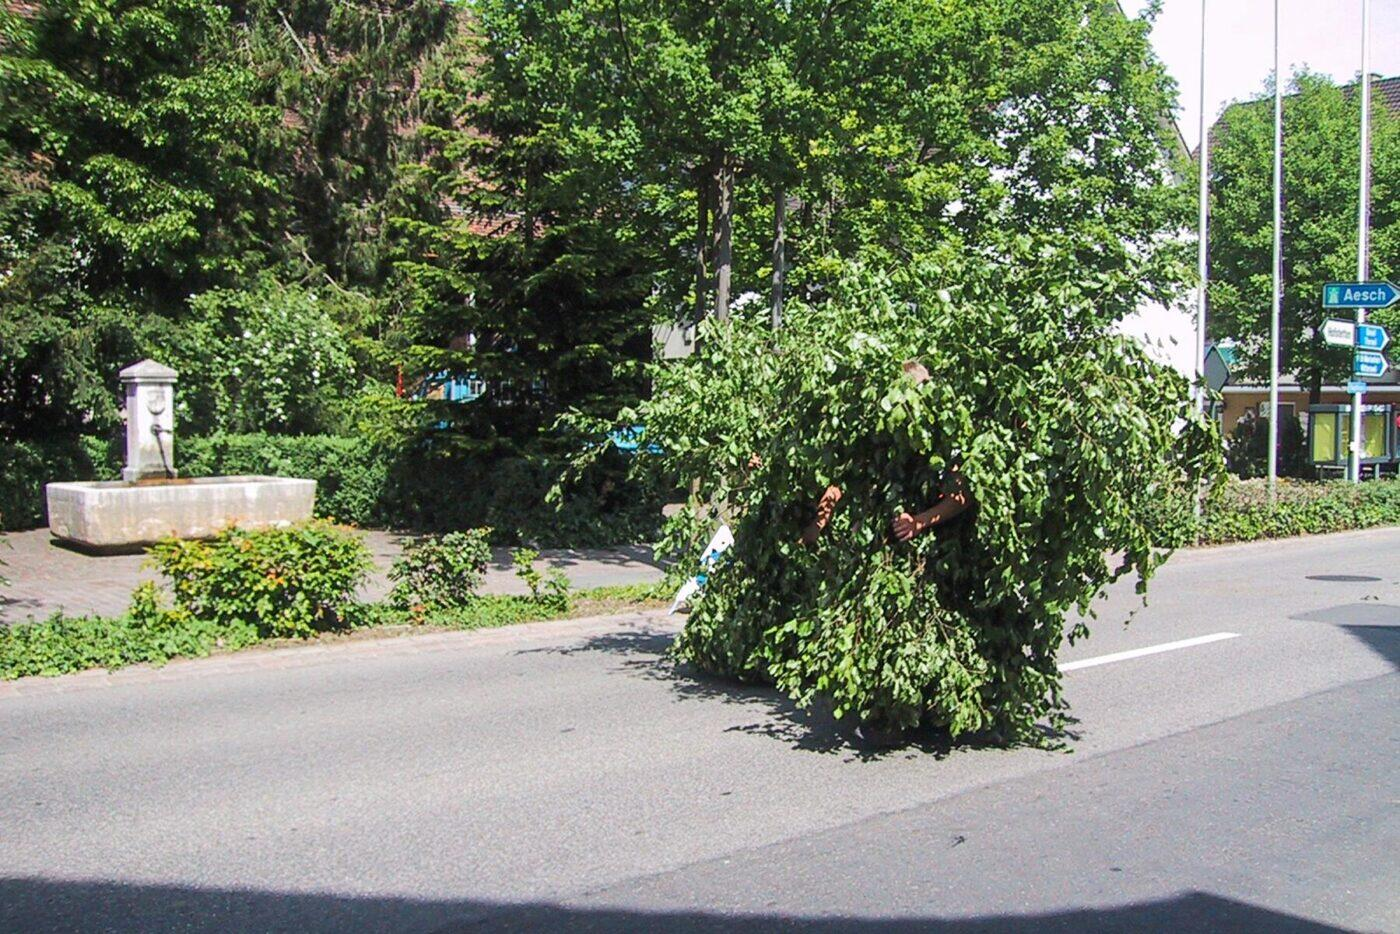
\includegraphics[width=\columnwidth]{images/bushes.jpg}}
      \only<5>{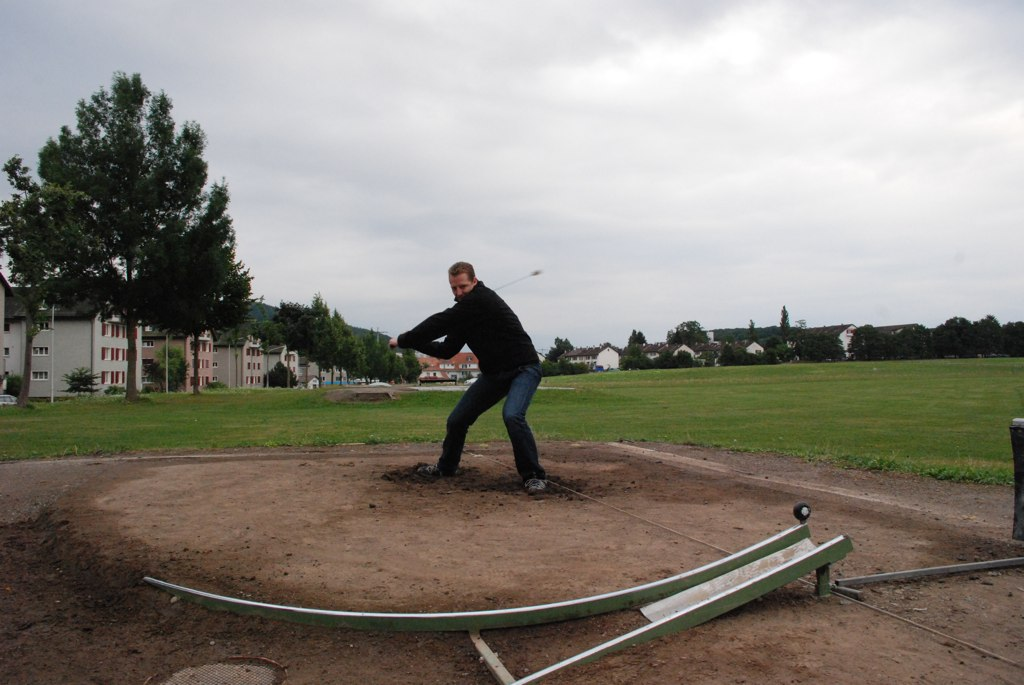
\includegraphics[width=\columnwidth]{images/Hornussen_Peschi.jpg}}
      \only<6>{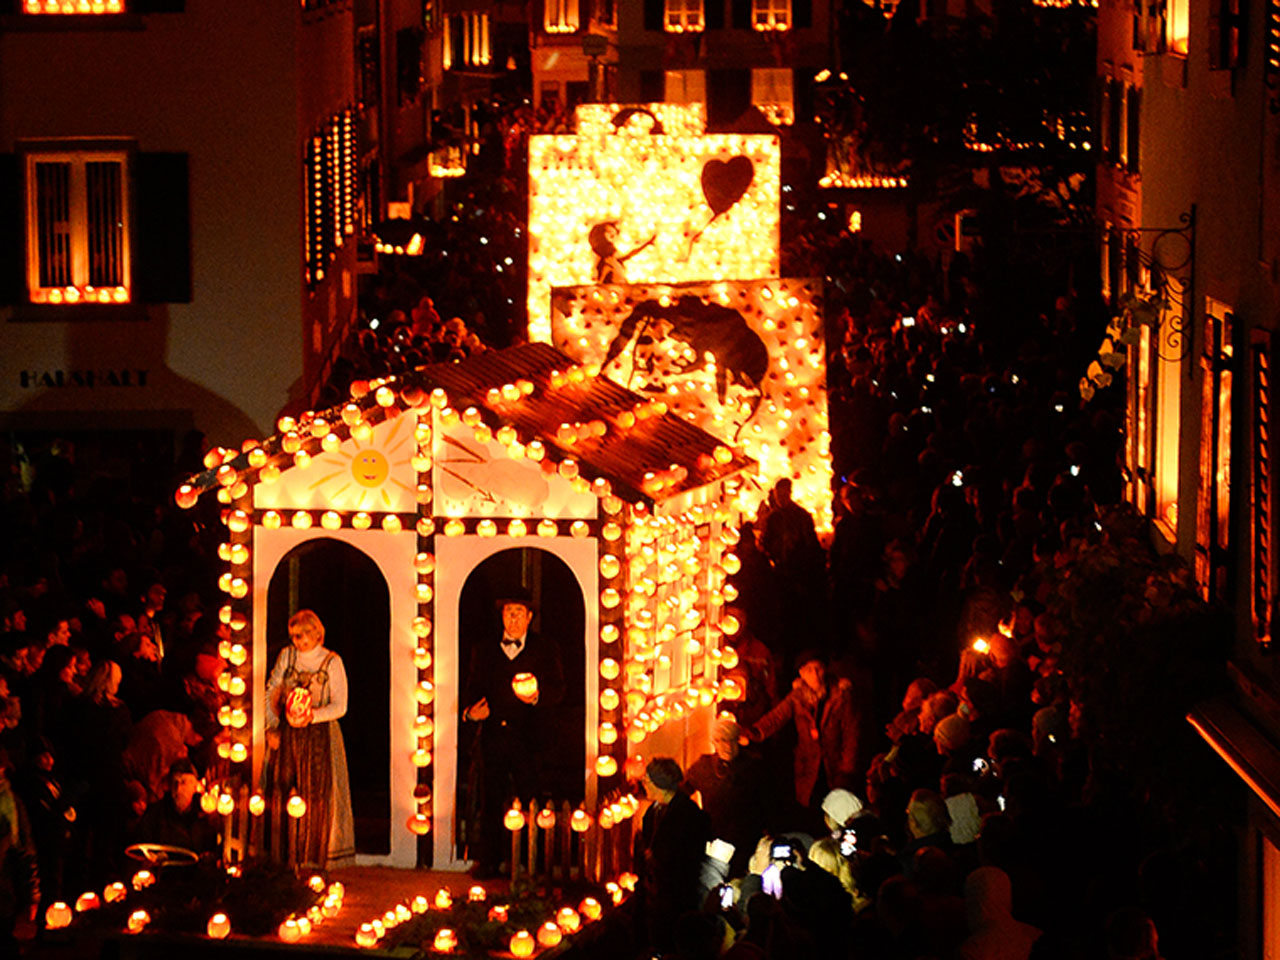
\includegraphics[width=\columnwidth]{images/turnip.jpg}}
   \end{overlayarea}
\end{column}
\end{columns}
\end{frame}
\begin{frame}
\begin{center}
\Huge
Round 2: ``Marvel''
\end{center}
\end{frame}
\begin{frame}
\begin{center}
\Large
1. Which popular hymn was written by a repentant ex-slave-ship owner?
\end{center}
\end{frame}
\begin{frame}
\begin{center}
\Large
2. In tennis, what feat was most recently achieved by Steffi Graf in 1988? (Here I am excluding wheelchair disciplines; it has been achieved three times by Diede de Groot since 2021.)
\end{center}
\end{frame}
\begin{frame}
\begin{center}
\Large
3. Which US National Park is this?
\\
\vspace{0.5em}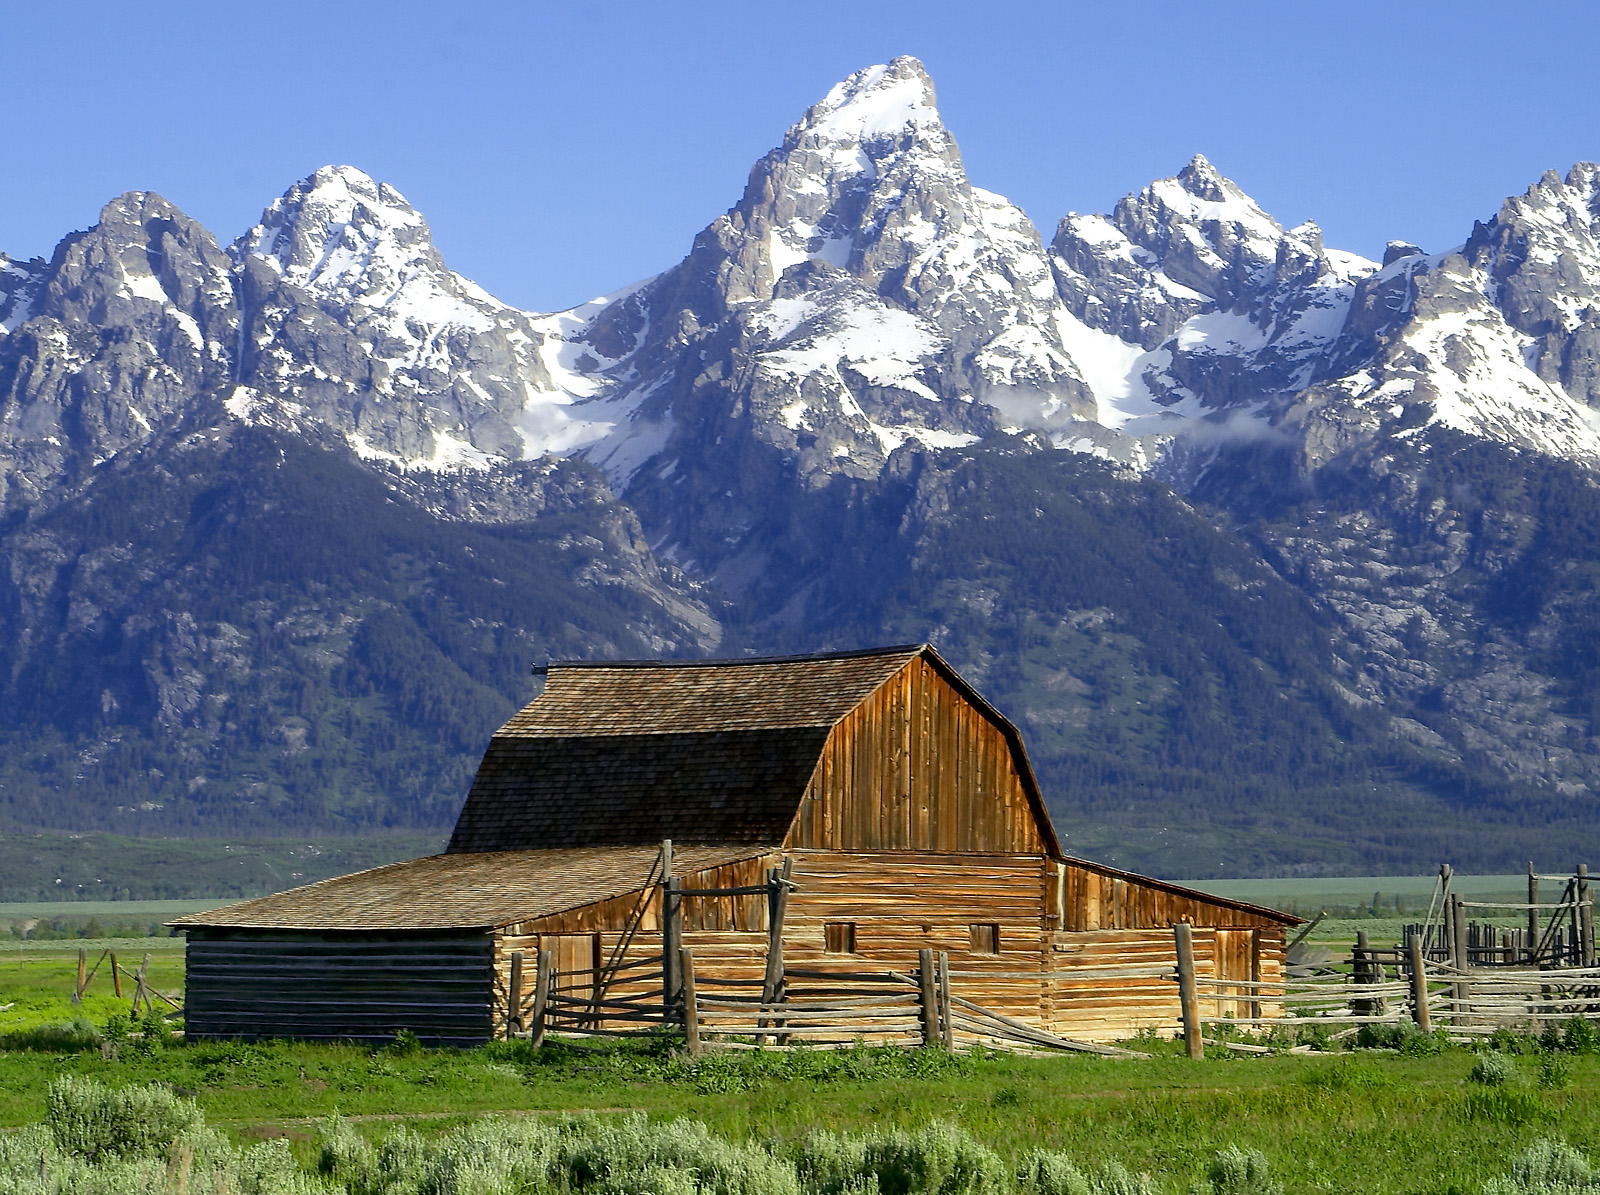
\includegraphics[height=0.6\paperheight]{images/grand_tetons.jpg}
\end{center}
\end{frame}
\begin{frame}
\begin{center}
\Large
4. According to the US Library of Congress, what is the most watched film of all time?
\end{center}
\end{frame}
\begin{frame}
\begin{center}
\Large
5. Behind only Minecraft, what is the second-best selling video game of all time?
\end{center}
\end{frame}
\begin{frame}
\begin{center}
\Large
6. What was the first song from the 1990s to reach a billion streams on Spotify?
\end{center}
\end{frame}
\begin{frame}
\begin{center}
\Large
7. Of all the MARVEL films, which has the lowest rating on Rotten Tomatoes? It was released in 2015.
\end{center}
\end{frame}
\begin{frame}
\begin{center}
\Huge
Answers
\end{center}
\end{frame}
\begin{frame}
\begin{center}
\Large
1. Which popular hymn was written by a repentant ex-slave-ship owner?
\\
\onslide<2->{\vspace{1em}\textit{Amazing Grace}}
\end{center}
\end{frame}
\begin{frame}
\begin{center}
\Large
2. In tennis, what feat was most recently achieved by Steffi Graf in 1988? (Here I am excluding wheelchair disciplines; it has been achieved three times by Diede de Groot since 2021.)
\\
\onslide<2->{\vspace{1em}\textit{a calendar Grand Slam in singles}}
\end{center}
\end{frame}
\begin{frame}
\begin{center}
\Large
3. Which US National Park is this?
\\
\vspace{0.5em}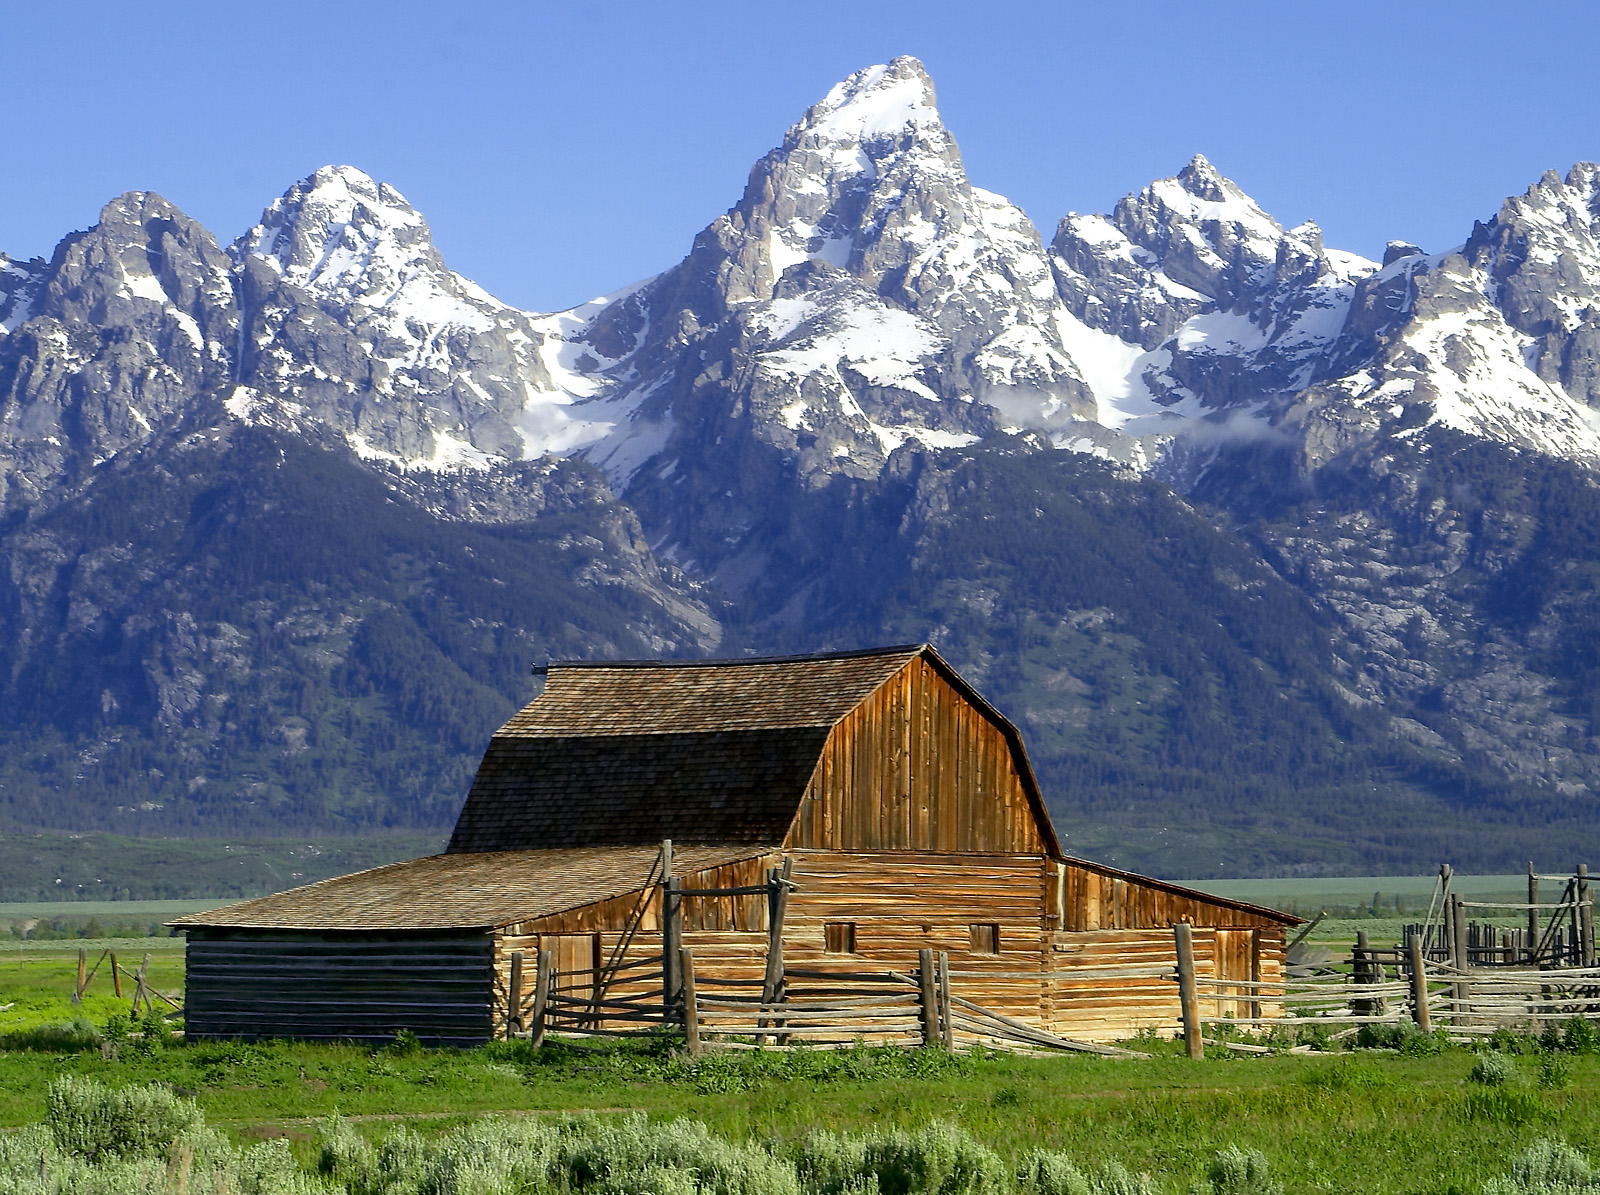
\includegraphics[height=0.6\paperheight]{images/grand_tetons.jpg}
\\
\onslide<2->{\vspace{1em}\textit{Grand Teton National Park}}
\end{center}
\end{frame}
\begin{frame}
\begin{center}
\Large
4. According to the US Library of Congress, what is the most watched film of all time?
\\
\onslide<2->{\vspace{1em}\textit{The (Wonderful) Wizard of Oz}}
\end{center}
\end{frame}
\begin{frame}
\begin{center}
\Large
5. Behind only Minecraft, what is the second-best selling video game of all time?
\\
\onslide<2->{\vspace{1em}\textit{Grand Theft Auto V}}
\end{center}
\end{frame}
\begin{frame}
\begin{center}
\Large
6. What was the first song from the 1990s to reach a billion streams on Spotify?
\\
\onslide<2->{\vspace{1em}\textit{Wonderwall (Oasis)}}
\end{center}
\end{frame}
\begin{frame}
\begin{center}
\Large
7. Of all the MARVEL films, which has the lowest rating on Rotten Tomatoes? It was released in 2015.
\\
\onslide<2->{\vspace{1em}\textit{Fantastic Four (a measly 9\%)}}
\end{center}
\end{frame}
\begin{frame}
\begin{center}
\Huge
Round 3: Design and Discovery of Novel Materials
\end{center}
\end{frame}
\begin{frame}
\begin{center}
\Large
1. What was the nationality of the first European explorer to discover New Zealand?
\end{center}
\end{frame}
\begin{frame}
\begin{center}
\Large
2. The Pritzker Prize is the most prestigious international prize in what field?
\end{center}
\end{frame}
\begin{frame}
\begin{center}
\Large
3. ``Prophet Song'', ``The Seven Moons of Maali Almeida'', and ``The Promise'' are all prize-winning whats?
\end{center}
\end{frame}
\begin{frame}
\begin{center}
\Large
4. gaberdine, lawn, brocade, and french terry are all examples of what?
\end{center}
\end{frame}
\begin{frame}
\begin{center}
\Large
5. In 2023, researchers discovered that the T-Rex had what body part? Its presence would make them appear much less scary.
\end{center}
\end{frame}
\begin{frame}
\begin{center}
\Large
6. In the context of philosphy, what is ``Materialism''
\end{center}
\end{frame}
\begin{frame}
\begin{center}
\Large
7. What is this famous building?
\\
\vspace{0.5em}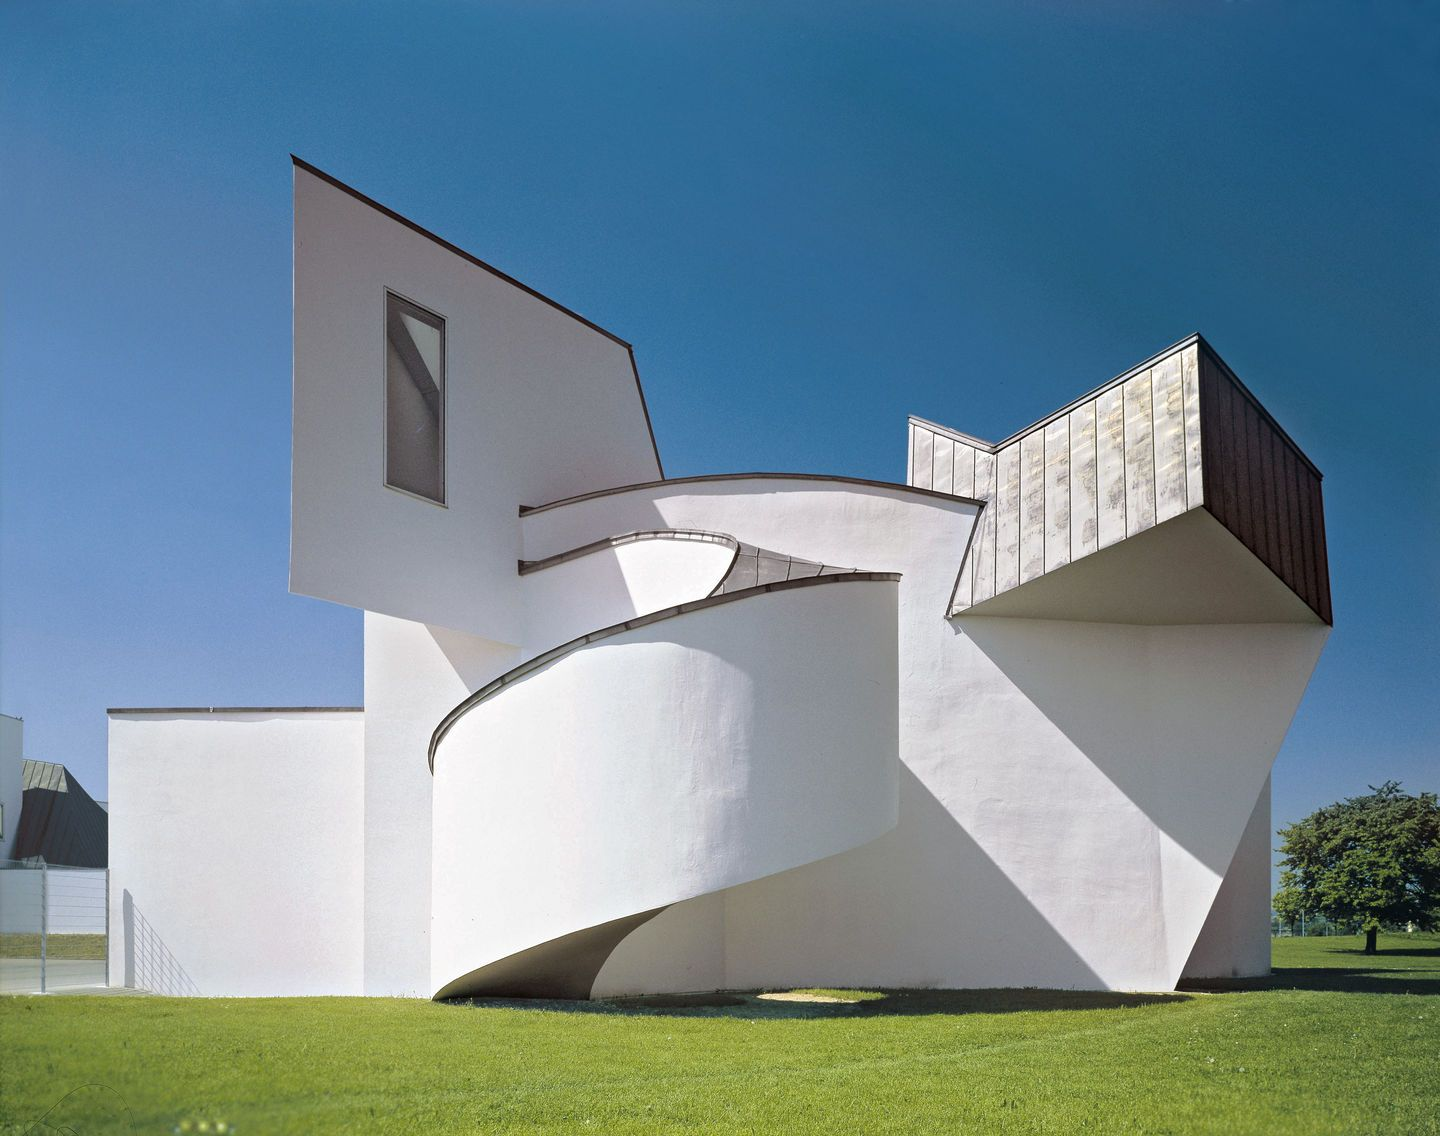
\includegraphics[height=0.6\paperheight]{images/vitra.jpg}
\end{center}
\end{frame}
\begin{frame}
\begin{center}
\Large
8. This is the opening verse to which song?
\begin{center}
    \begin{minipage}{0.6\textwidth}
        \textit{%
            Some boys kiss me \\
            Some boys hug me \\
            I think they're ok \\
            If they don't give me proper credit \\
            I just walk away}%
    \end{minipage}
\end{center}

\end{center}
\end{frame}
\begin{frame}
\begin{center}
\Huge
Answers
\end{center}
\end{frame}
\begin{frame}
\begin{center}
\Large
1. What was the nationality of the first European explorer to discover New Zealand?
\\
\onslide<2->{\vspace{1em}\textit{Dutch}}
\end{center}
\end{frame}
\begin{frame}
\begin{center}
\Large
2. The Pritzker Prize is the most prestigious international prize in what field?
\\
\onslide<2->{\vspace{1em}\textit{Architecture}}
\end{center}
\end{frame}
\begin{frame}
\begin{center}
\Large
3. ``Prophet Song'', ``The Seven Moons of Maali Almeida'', and ``The Promise'' are all prize-winning whats?
\\
\onslide<2->{\vspace{1em}\textit{Novels -- in fact, they are the three most recent Booker Prize winners}}
\end{center}
\end{frame}
\begin{frame}
\begin{center}
\Large
4. gaberdine, lawn, brocade, and french terry are all examples of what?
\\
\onslide<2->{\vspace{1em}\textit{fabrics}}
\end{center}
\end{frame}
\begin{frame}
\begin{center}
\Large
5. In 2023, researchers discovered that the T-Rex had what body part? Its presence would make them appear much less scary.
\\
\onslide<2->{\vspace{1em}\textit{lips}}
\end{center}
\end{frame}
\begin{frame}
\begin{center}
\Large
6. In the context of philosphy, what is ``Materialism''
\\
\onslide<2->{\vspace{1em}\textit{The theory in which physical matter is the only reality and that all being, processes, and phenomena can be explained as manifestations or results of matter}}
\end{center}
\end{frame}
\begin{frame}
\begin{center}
\Large
7. What is this famous building?
\\
\vspace{0.5em}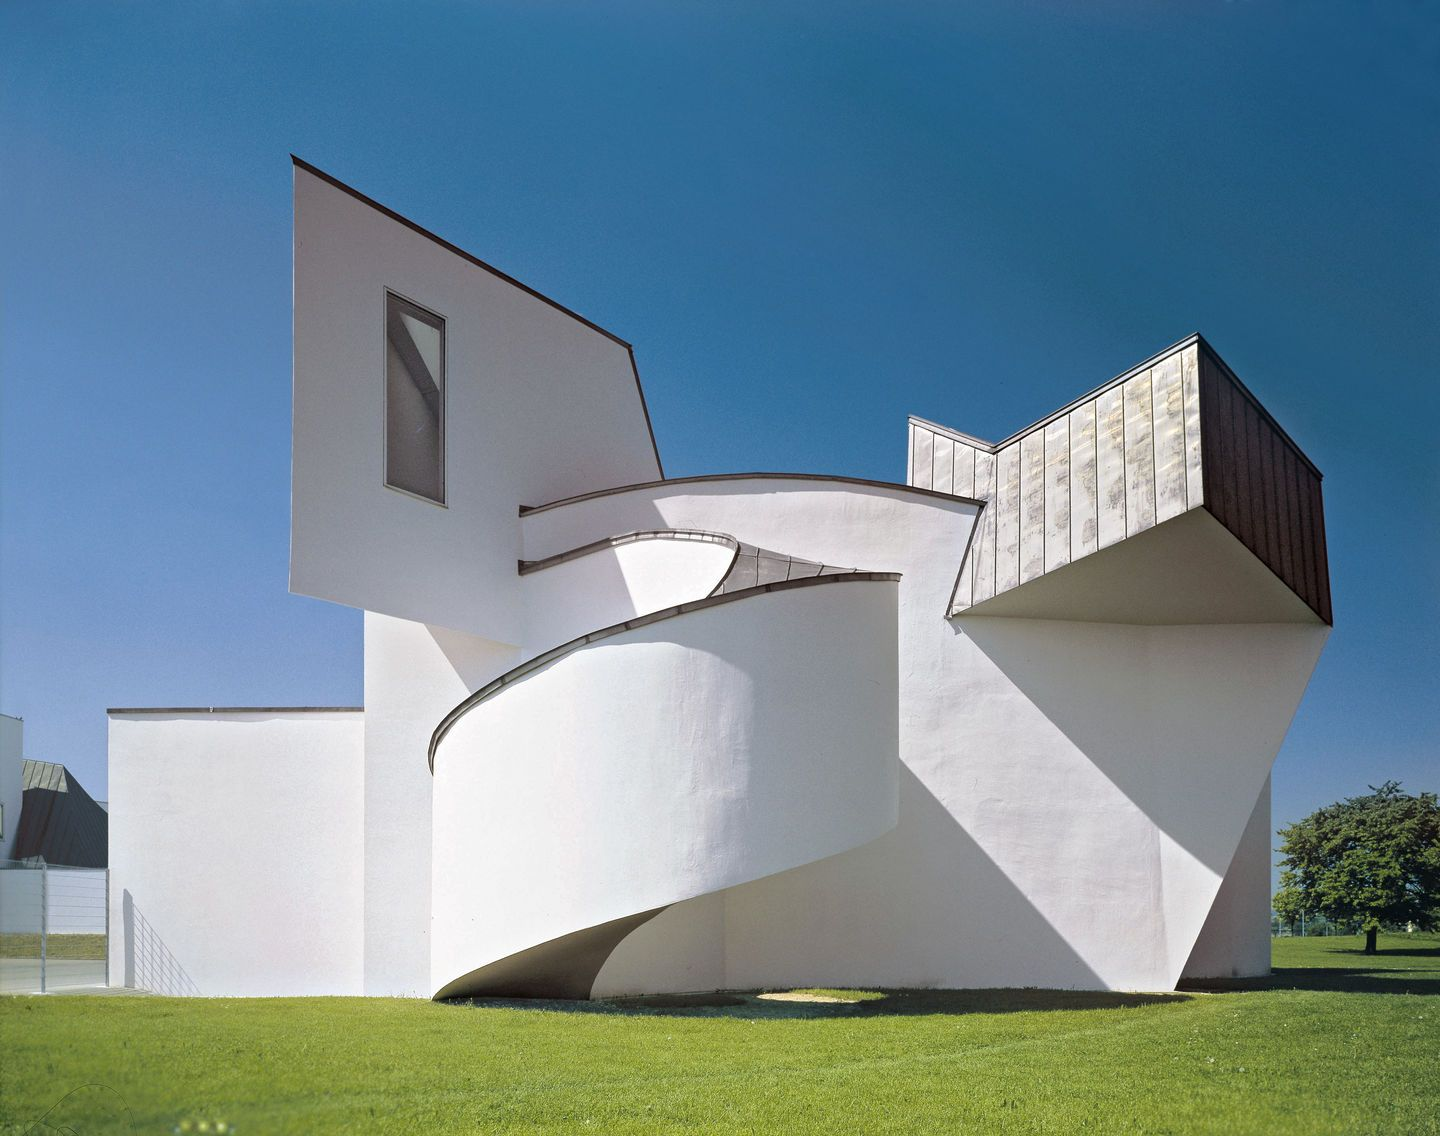
\includegraphics[height=0.6\paperheight]{images/vitra.jpg}
\\
\onslide<2->{\vspace{1em}\textit{Vitra Design Museum (Basel)}}
\end{center}
\end{frame}
\begin{frame}
\begin{center}
\Large
8. This is the opening verse to which song?
\begin{center}
    \begin{minipage}{0.6\textwidth}
        \textit{%
            Some boys kiss me \\
            Some boys hug me \\
            I think they're ok \\
            If they don't give me proper credit \\
            I just walk away}%
    \end{minipage}
\end{center}

\onslide<2->{\vspace{1em}\textit{Material Girl (Madonna)}}
\end{center}
\end{frame}
\begin{frame}
\begin{center}
\Huge
Round 4: Changing things up
\end{center}
\end{frame}
\begin{frame}
\begin{center}
\Large
1. ?
\end{center}
\end{frame}
\begin{frame}
\begin{center}
\Large
2. Which 2023 TV series was widely ridiculed because it featured ghosts?
\end{center}
\end{frame}
\begin{frame}
\begin{center}
\Large
3. Film with dollar in the title e.g. Which film pipped The Aviator to best picture in 2004?
\end{center}
\end{frame}
\begin{frame}
\begin{center}
\Large
4. ?
\end{center}
\end{frame}
\begin{frame}
\begin{center}
\Large
5. What kind of dog is this?
\\
\vspace{0.5em}
\includegraphics[height=0.6\paperheight]{images/doge.jpg}
\end{center}
\end{frame}
\begin{frame}
\begin{center}
\Large
6. What major sporting tournament is being held in Germany later this year?
\end{center}
\end{frame}
\begin{frame}
\begin{center}
\Large
7. Who wrote "Atlas Shrugged"? It is a novel that is very influential in libertarian and conservative circles, especially in America
\end{center}
\end{frame}
\begin{frame}
\begin{center}
\Large
8. What links the answers to all the questions in this round?
\end{center}
\end{frame}
\begin{frame}
\begin{center}
\Huge
Answers
\end{center}
\end{frame}
\begin{frame}
\begin{center}
\Large
1. ?
\\
\onslide<2->{\vspace{1em}\textit{Franc someone? (Francis Drake)}}
\end{center}
\end{frame}
\begin{frame}
\begin{center}
\Large
2. Which 2023 TV series was widely ridiculed because it featured ghosts?
\\
\onslide<2->{\vspace{1em}\textit{The Crown}}
\end{center}
\end{frame}
\begin{frame}
\begin{center}
\Large
3. Film with dollar in the title e.g. Which film pipped The Aviator to best picture in 2004?
\\
\onslide<2->{\vspace{1em}\textit{Million Dollar Baby -- not a great question}}
\end{center}
\end{frame}
\begin{frame}
\begin{center}
\Large
4. ?
\\
\onslide<2->{\vspace{1em}\textit{Centurion}}
\end{center}
\end{frame}
\begin{frame}
\begin{center}
\Large
5. What kind of dog is this?
\\
\vspace{0.5em}
\includegraphics[height=0.6\paperheight]{images/doge.jpg}
\\
\onslide<2->{\vspace{1em}\textit{a Shiba Inu}}
\end{center}
\end{frame}
\begin{frame}
\begin{center}
\Large
6. What major sporting tournament is being held in Germany later this year?
\\
\onslide<2->{\vspace{1em}\textit{The Euros}}
\end{center}
\end{frame}
\begin{frame}
\begin{center}
\Large
7. Who wrote "Atlas Shrugged"? It is a novel that is very influential in libertarian and conservative circles, especially in America
\\
\onslide<2->{\vspace{1em}\textit{Ayn Rand}}
\end{center}
\end{frame}
\begin{frame}
\begin{center}
\Large
8. What links the answers to all the questions in this round?
\\
\onslide<2->{\vspace{1em}\textit{currencies}}
\end{center}
\end{frame}
\begin{frame}
\begin{center}
\Huge
Round 5: Numbers
\end{center}
\end{frame}
\begin{frame}
\begin{center}
\Large
1. How many times will Halley's comet transit earth in the 21st century?
\end{center}
\end{frame}
\begin{frame}
\begin{center}
\Large
2. How many eyelids (per eye) does a polar bear have?
\end{center}
\end{frame}
\begin{frame}
\begin{center}
\Large
3. Osmium is how many times more dense than lead? It is the densest material nautrally found on earth.
\end{center}
\end{frame}
\begin{frame}
\begin{center}
\Large
4. How many many Pirates of the Caribbean films are there?
\end{center}
\end{frame}
\begin{frame}
\begin{center}
\Large
5. In handball, how many players does one team have (excluding subs)?
\end{center}
\end{frame}
\begin{frame}
\begin{center}
\Large
6. Rounded to the nearest whole number, how many kilograms are there in 1 stone?
\end{center}
\end{frame}
\begin{frame}
\begin{center}
\Large
7. From takeoff to splashdown, how many days long was the Apollo 11 mission?
\end{center}
\end{frame}
\begin{frame}
\begin{center}
\Large
8. At 1200m, how many degrees below 100\textdegree C does water boil? (We are currently at 1050m.)
\end{center}
\end{frame}
\begin{frame}
\begin{center}
\Huge
Answers
\end{center}
\end{frame}
\begin{frame}
\begin{center}
\Large
1. How many times will Halley's comet transit earth in the 21st century?
\\
\onslide<2->{\vspace{1em}\textit{1 (it is visible every 75 or so years, and will next appear in mid-2061)}}
\end{center}
\end{frame}
\begin{frame}
\begin{center}
\Large
2. How many eyelids (per eye) does a polar bear have?
\\
\onslide<2->{\vspace{1em}\textit{3}}
\end{center}
\end{frame}
\begin{frame}
\begin{center}
\Large
3. Osmium is how many times more dense than lead? It is the densest material nautrally found on earth.
\\
\onslide<2->{\vspace{1em}\textit{2}}
\end{center}
\end{frame}
\begin{frame}
\begin{center}
\Large
4. How many many Pirates of the Caribbean films are there?
\\
\onslide<2->{\vspace{1em}\textit{5}}
\end{center}
\end{frame}
\begin{frame}
\begin{center}
\Large
5. In handball, how many players does one team have (excluding subs)?
\\
\onslide<2->{\vspace{1em}\textit{7}}
\end{center}
\end{frame}
\begin{frame}
\begin{center}
\Large
6. Rounded to the nearest whole number, how many kilograms are there in 1 stone?
\\
\onslide<2->{\vspace{1em}\textit{6}}
\end{center}
\end{frame}
\begin{frame}
\begin{center}
\Large
7. From takeoff to splashdown, how many days long was the Apollo 11 mission?
\\
\onslide<2->{\vspace{1em}\textit{8}}
\end{center}
\end{frame}
\begin{frame}
\begin{center}
\Large
8. At 1200m, how many degrees below 100\textdegree C does water boil? (We are currently at 1050m.)
\\
\onslide<2->{\vspace{1em}\textit{4}}
\end{center}
\end{frame}
\begin{frame}
\begin{center}
\Huge
Pictures: Sizing up the world
\end{center}
\end{frame}
\begin{frame}
\begin{center}
\Large
1. 
\\
\vspace{0.5em}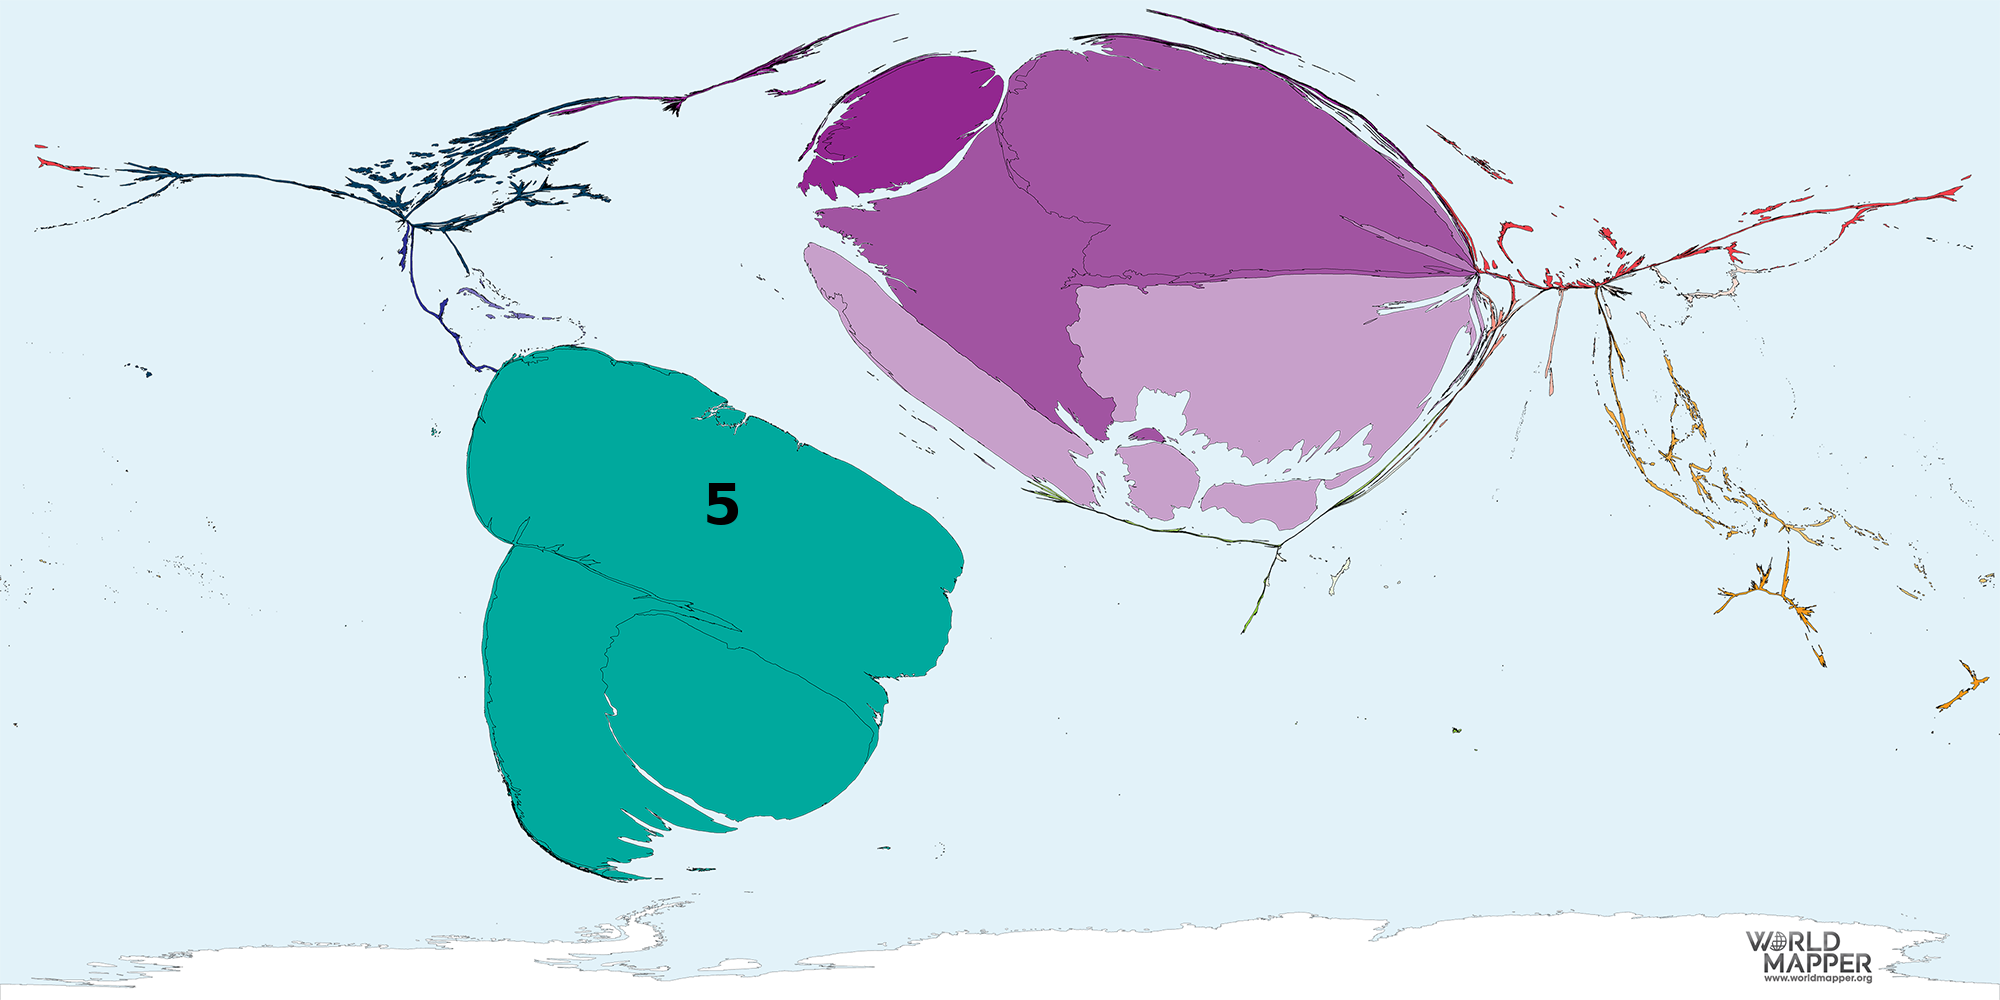
\includegraphics[height=0.6\paperheight]{maps/picture_1.png}
\\
\onslide<2->{\vspace{1em}\textit{GDP (purchasing-parity-power-adjusted)}}
\end{center}
\end{frame}
\begin{frame}
\begin{center}
\Large
2. 
\\
\vspace{0.5em}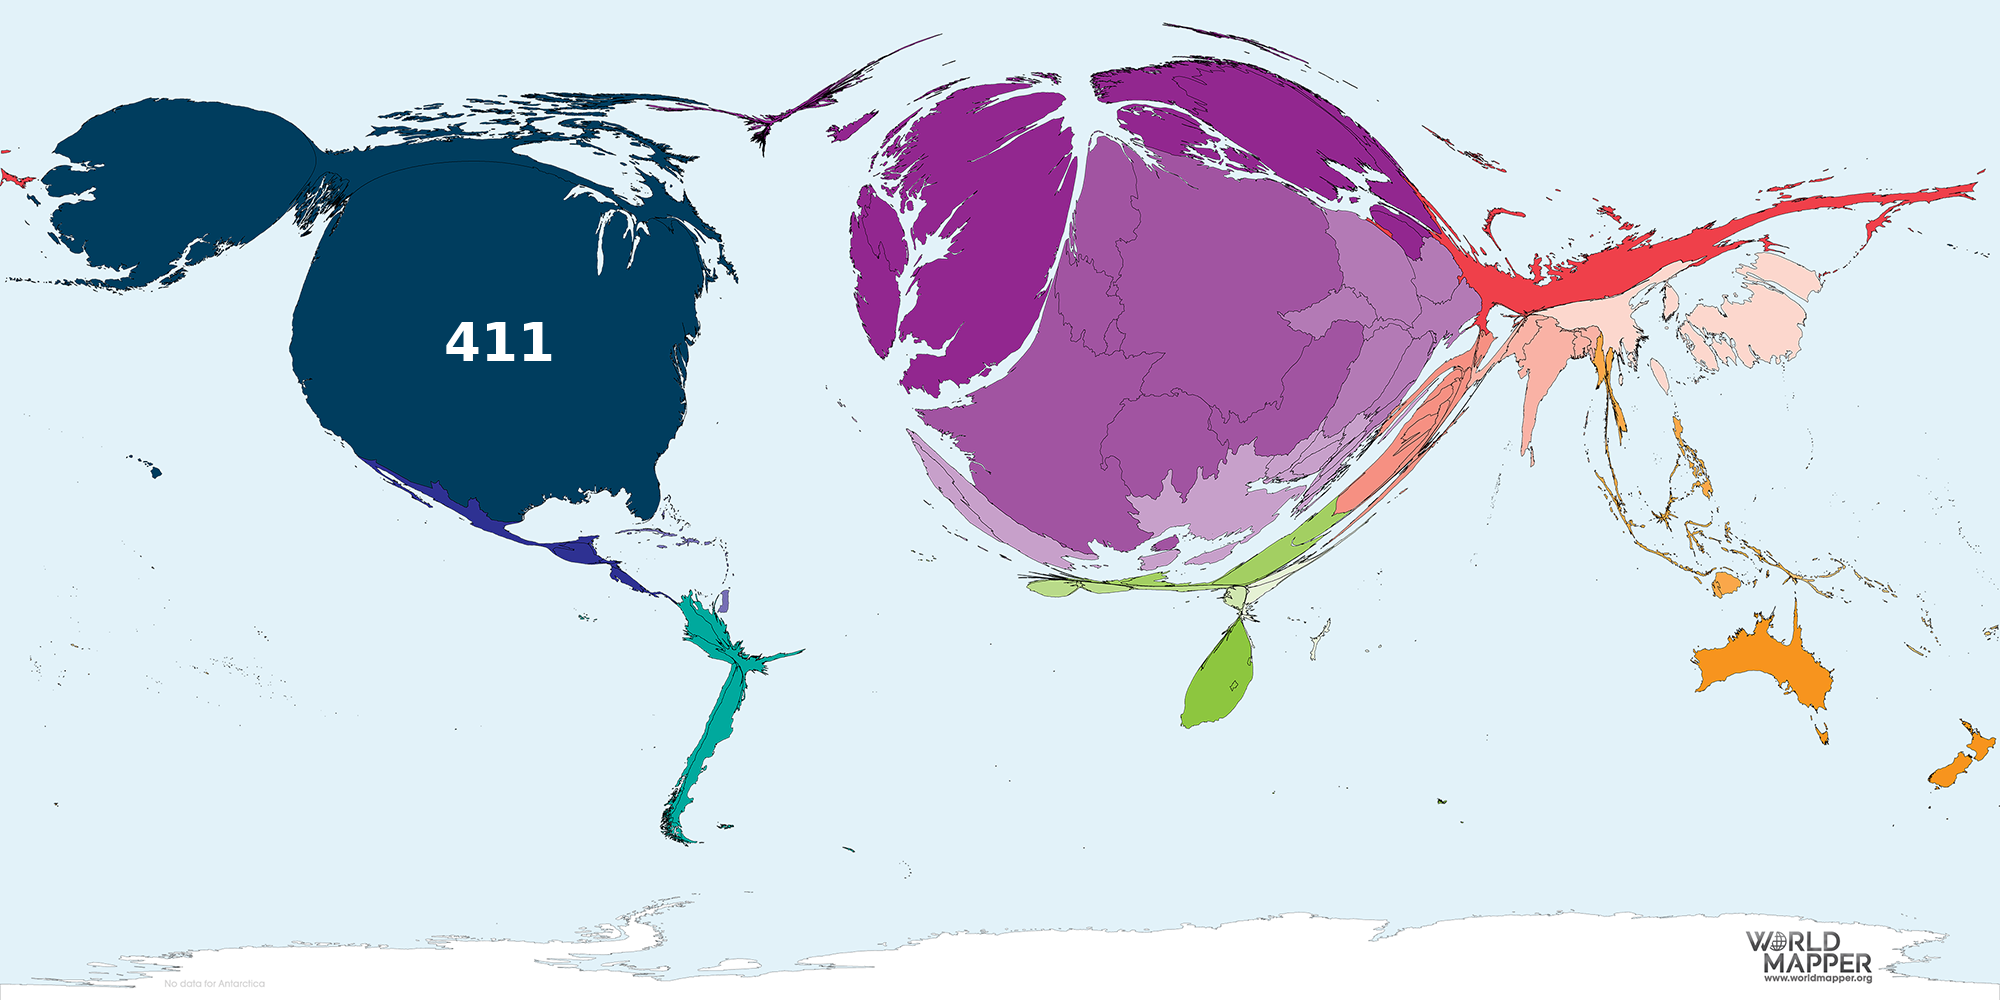
\includegraphics[height=0.6\paperheight]{maps/picture_2.png}
\\
\onslide<2->{\vspace{1em}\textit{Nobel laureates}}
\end{center}
\end{frame}
\begin{frame}
\begin{center}
\Large
3. 
\\
\vspace{0.5em}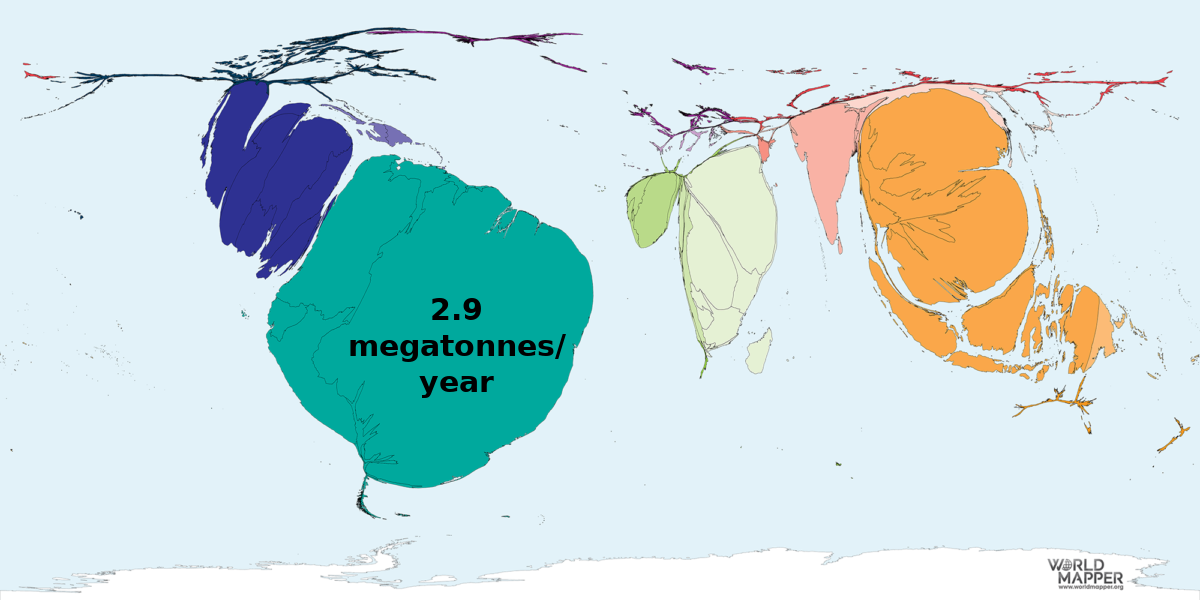
\includegraphics[height=0.6\paperheight]{maps/picture_3.png}
\\
\onslide<2->{\vspace{1em}\textit{coffee production}}
\end{center}
\end{frame}
\begin{frame}
\begin{center}
\Large
4. 
\\
\vspace{0.5em}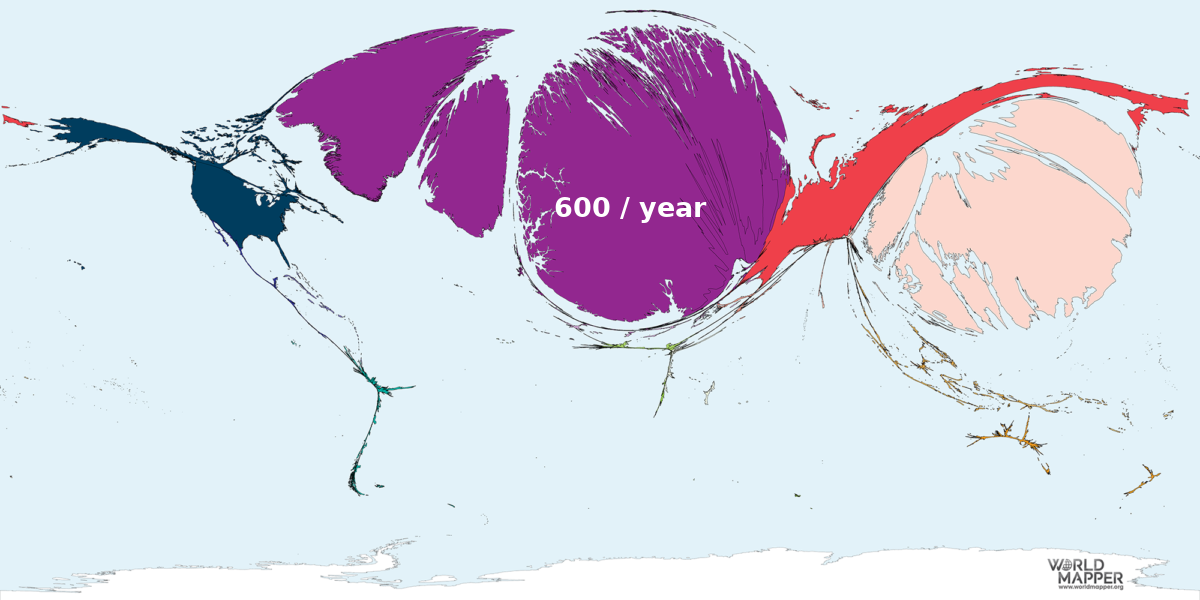
\includegraphics[height=0.6\paperheight]{maps/picture_4.png}
\\
\onslide<2->{\vspace{1em}\textit{whales killed}}
\end{center}
\end{frame}
\begin{frame}
\begin{center}
\Large
5. 
\\
\vspace{0.5em}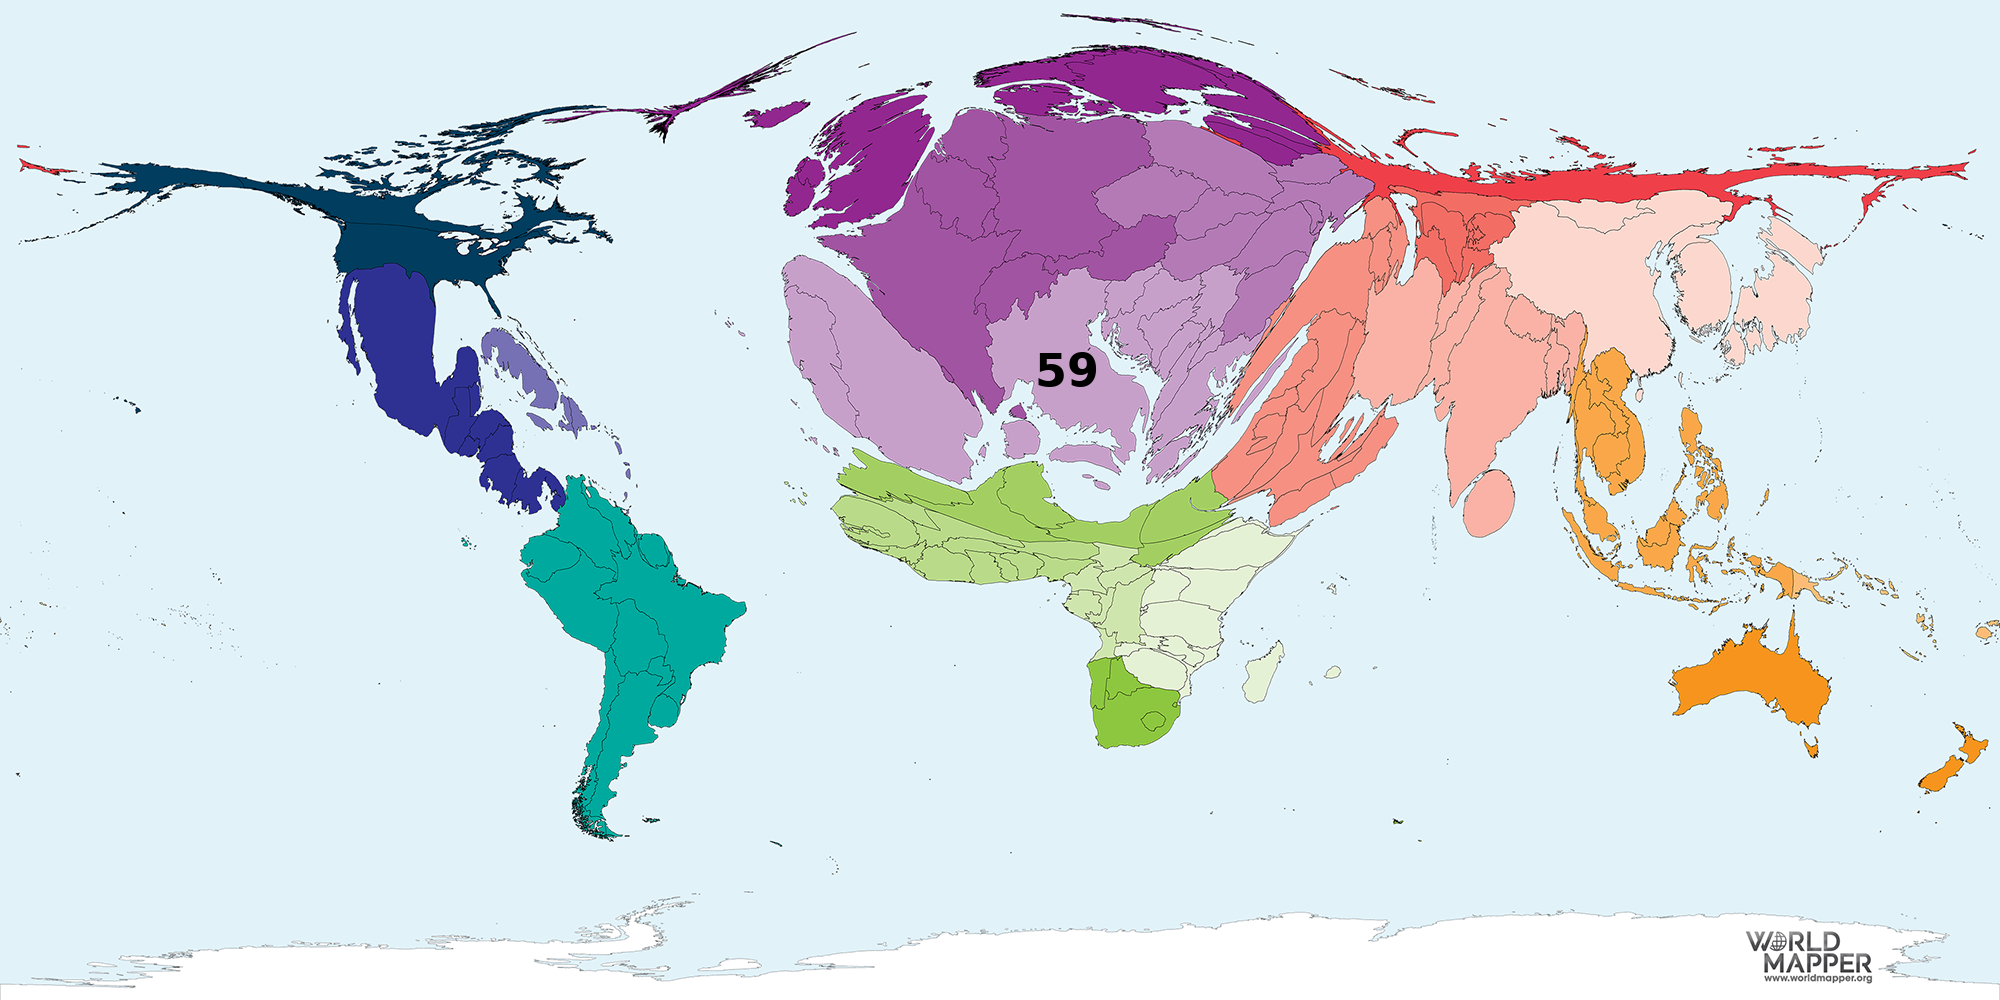
\includegraphics[height=0.6\paperheight]{maps/picture_5.png}
\\
\onslide<2->{\vspace{1em}\textit{population}}
\end{center}
\end{frame}
\begin{frame}
\begin{center}
\Large
6. 
\\
\vspace{0.5em}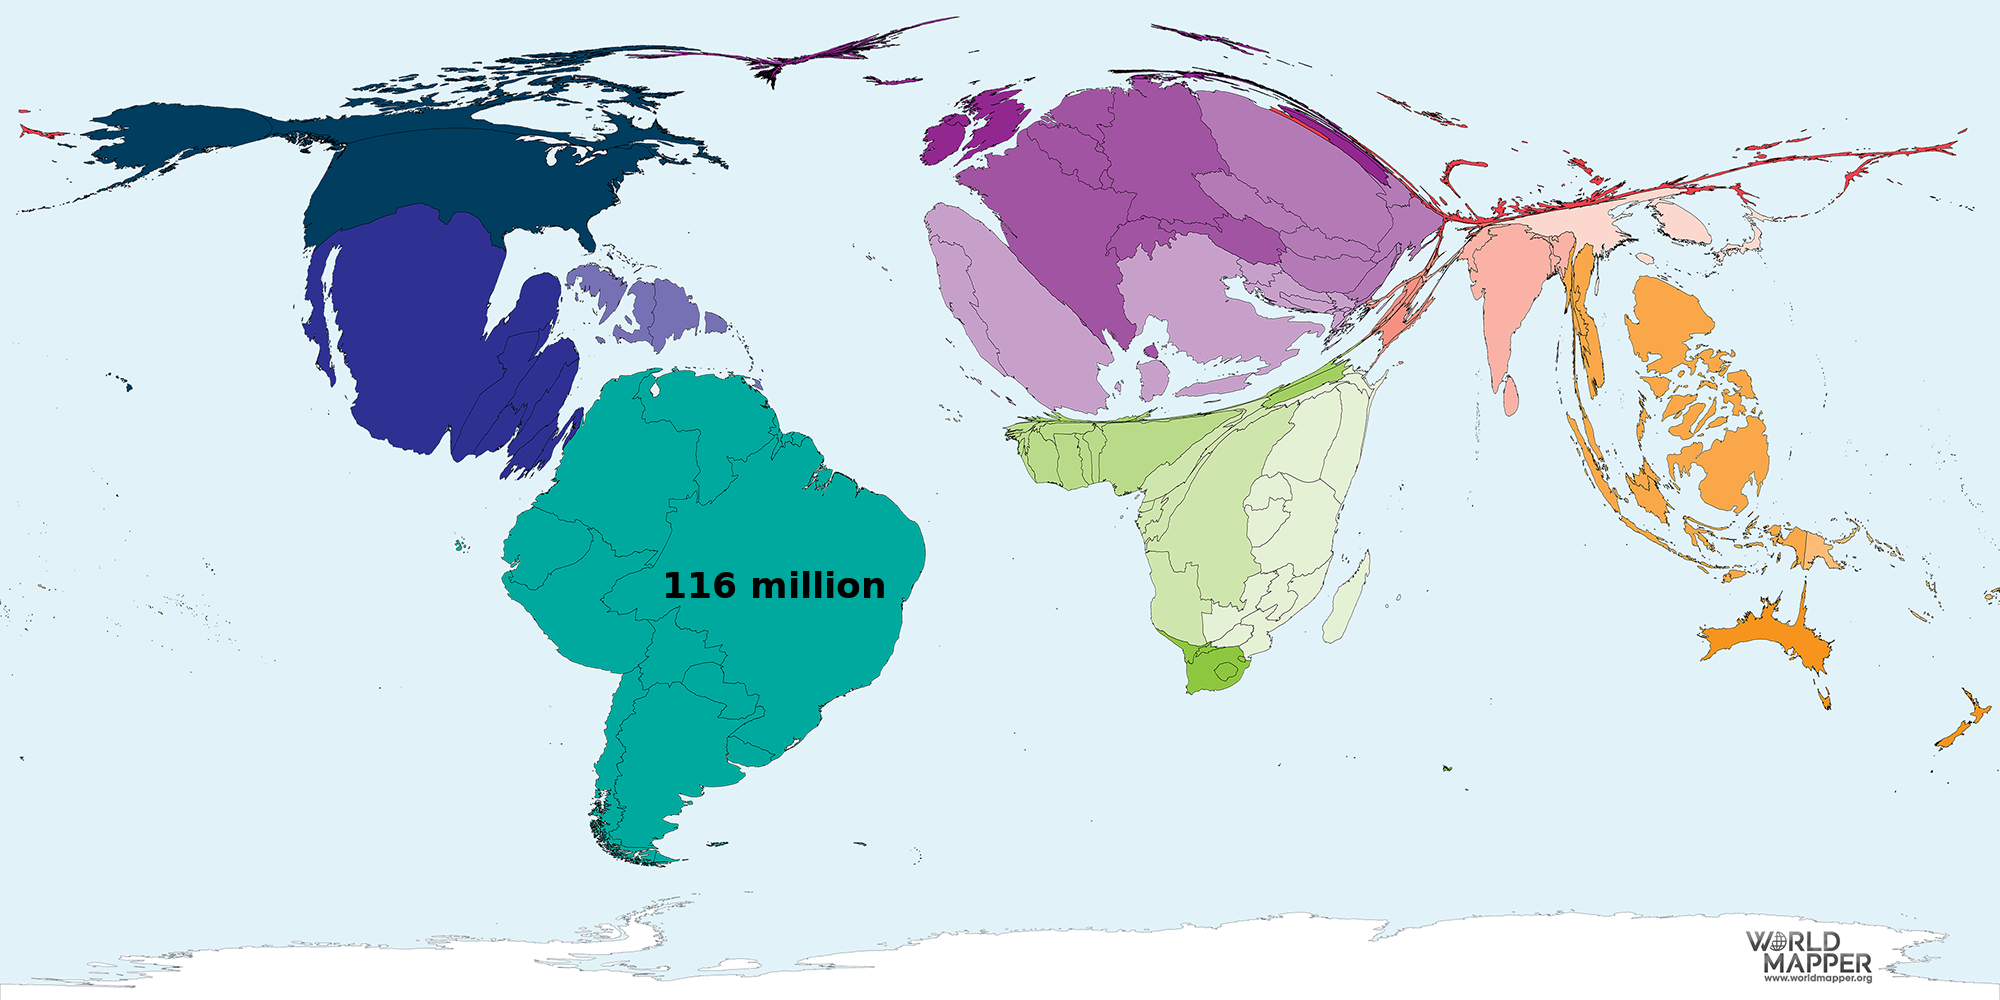
\includegraphics[height=0.6\paperheight]{maps/picture_6.png}
\\
\onslide<2->{\vspace{1em}\textit{number of Catholics}}
\end{center}
\end{frame}
\begin{frame}
\begin{center}
\Large
7. 
\\
\vspace{0.5em}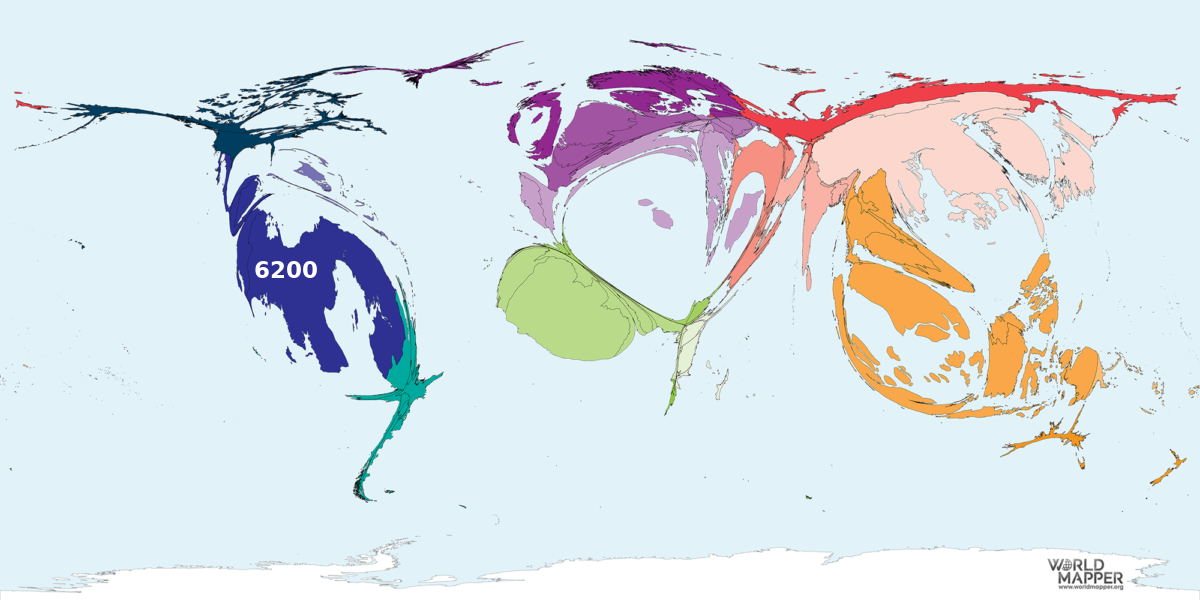
\includegraphics[height=0.6\paperheight]{maps/picture_7.png}
\\
\onslide<2->{\vspace{1em}\textit{number of registered ships}}
\end{center}
\end{frame}
\begin{frame}
\begin{center}
\Large
8. 
\\
\vspace{0.5em}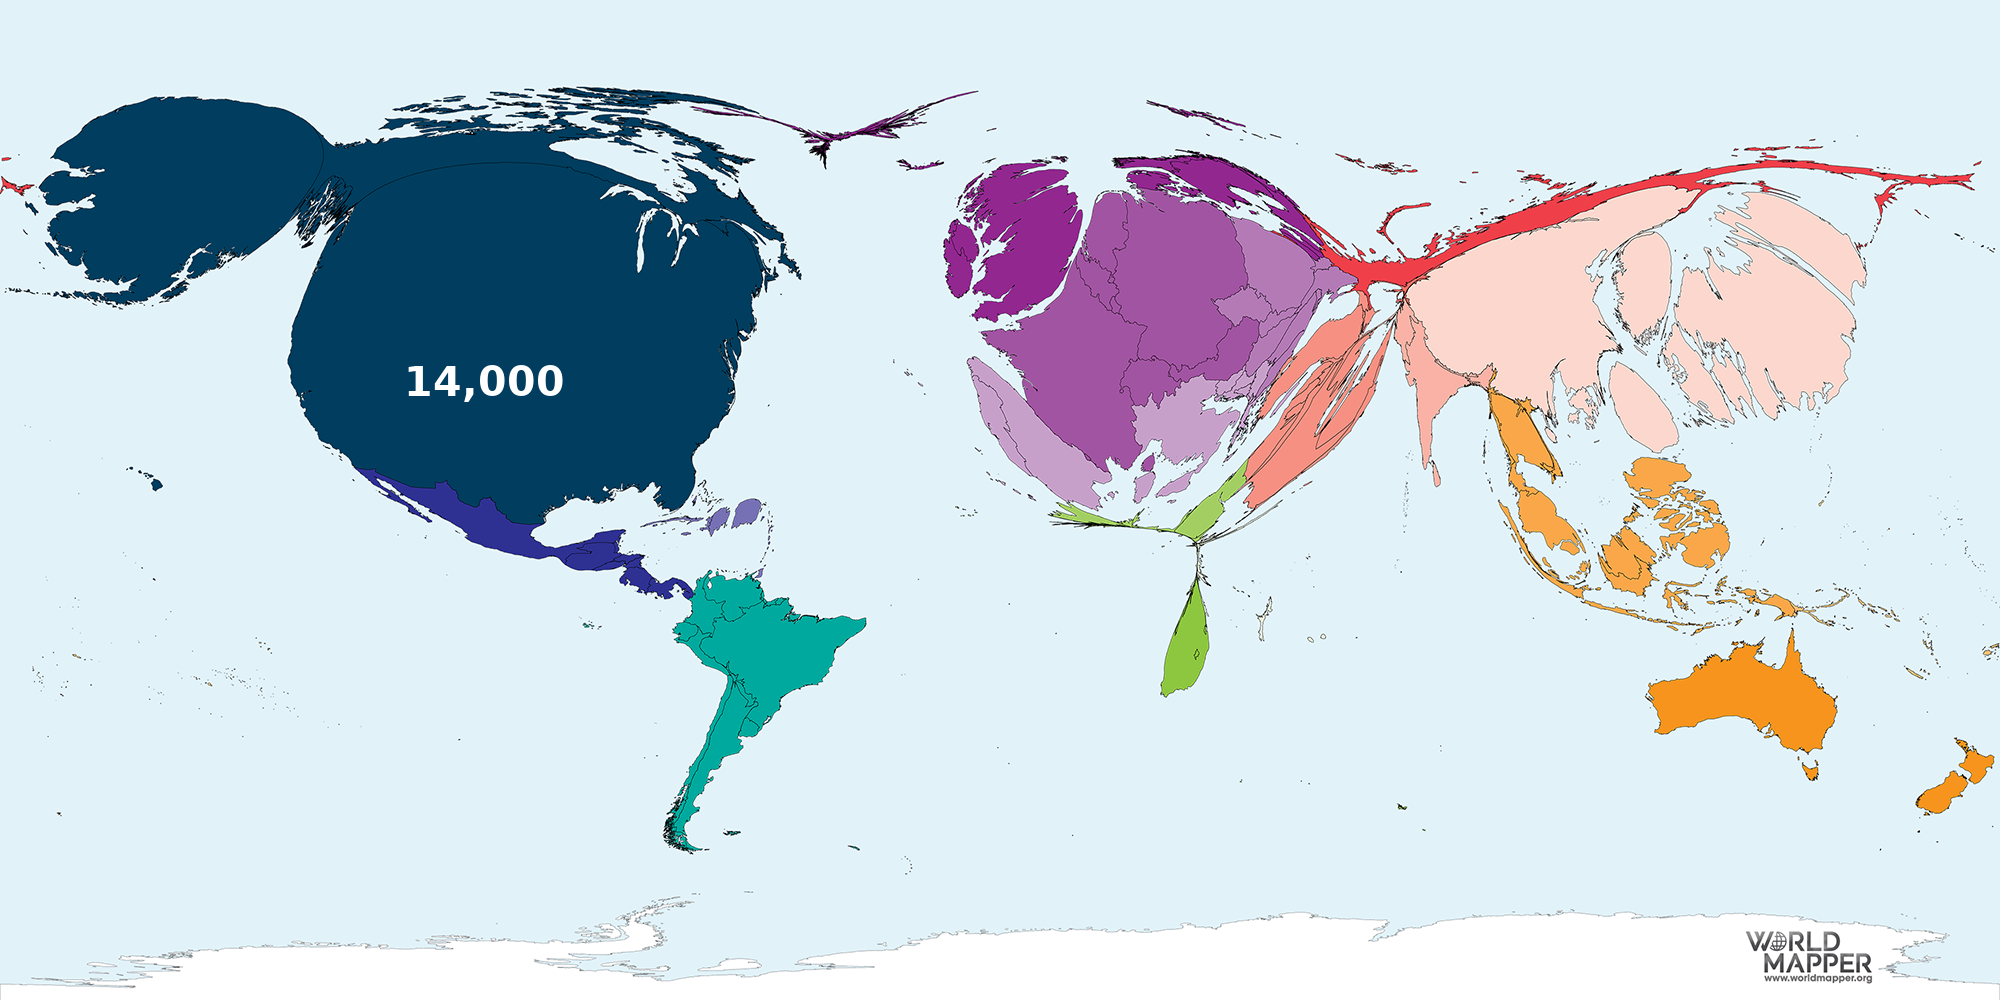
\includegraphics[height=0.6\paperheight]{maps/picture_8.png}
\\
\onslide<2->{\vspace{1em}\textit{number of McDonalds}}
\end{center}
\end{frame}
\begin{frame}
\begin{center}
\Huge
Puzzles: Connect Four
\end{center}
\end{frame}
\begin{frame}
\begin{center}
\Large
1. \leavevmode \\
\begin{center}
    \begin{minipage}{0.6\textwidth}
        \textit{%
            sharp taste \\
            words set to music \\
            Solo character \\
            archenemy of Flash Gordon}%
    \end{minipage}
\end{center}

\onslide<2->{\vspace{1em}\textit{Tang, Song, Han, and Ming: all Chinese dynasties}}
\end{center}
\end{frame}
\begin{frame}
\begin{center}
\Large
2. \leavevmode \\
\begin{center}
\setchessboard{boardfontsize=8pt, labelleft=false, labelbottom=false} % , labelfontsize=6pt
\newgame
\chessboard[setfen=4K3/8/8/8/8/8/8/8 w - - 0 0,showmover=False]
\chessboard[setfen=8/8/6K1/8/8/8/8/8 w - - 0 0,showmover=False]
\chessboard[setfen=8/8/8/8/8/8/4Q3/8 w - - 0 0,showmover=False]
\chessboard[setfen=8/8/8/8/8/2K5/8/8 w - - 0 0,showmover=False]
\end{center}
\onslide<2->{\vspace{1em}\textit{Ke8, Kg6, Qe2, and Kc3: British monarchs (Edward VIII, George VI, Elizabeth II, and Charles III)}}
\end{center}
\end{frame}
\begin{frame}
\begin{center}
\Large
3. \leavevmode \\
\begin{center}
    \begin{minipage}{0.6\textwidth}
        \textit{%
            a pew, Mr. Cuban, is a standard \\
            an entrance room, Mr. Cavendish, is a cheesy movie \\
            a profession, Mr. Twain, is a type of intellectual property \\
            a country, Mr. Hamill, is a monument}%
    \end{minipage}
\end{center}

\onslide<2->{\vspace{1em}\textit{benchmark, hallmark, trademark, and landmark}}
\end{center}
\end{frame}
\begin{frame}
\begin{center}
\Large
4. \leavevmode \\
\begin{center}
    \begin{minipage}{0.6\textwidth}
        \textit{%
            Test: objection and competition \\
            Found: deep and confuse \\
            Tract: extend and agreement \\
            Duct: goods and behaviour}%
    \end{minipage}
\end{center}

\onslide<2->{\vspace{1em}\textit{pros and cons}}
\end{center}
\end{frame}
\end{document}